\documentclass[letterpaper,11pt]{article}

\usepackage{ucs}
\usepackage[utf8x]{inputenc}
\usepackage{graphicx}
\usepackage{amsfonts}
\usepackage{dsfont}
\usepackage{amssymb}
\usepackage{amsmath}
\usepackage{amsthm}
\usepackage[titletoc]{appendix}

\usepackage{enumerate}
\usepackage{stmaryrd}
\usepackage{fullpage}
\usepackage{ifthen}
\usepackage{subfigure}
\usepackage{epic}
\usepackage{authblk}
\usepackage{textcomp}
\usepackage[small]{caption}
\SetSymbolFont{stmry}{bold}{U}{stmry}{m}{n}

\usepackage{enumitem}

\usepackage[hypertexnames=false,colorlinks=true,linkcolor=blue,citecolor=blue]{hyperref}
\usepackage[numbers,comma,square,sort&compress]{natbib}
\usepackage[letterpaper,text={7in,9in},centering]{geometry}

\usepackage{bm}
\usepackage{color}
\usepackage{titlesec}
\setlength{\parindent}{0.0in}
\setlength{\parskip}{1.0ex plus0.2ex minus0.2ex}
\renewcommand{\baselinestretch}{1.1}
\graphicspath{{eps/}{pdf/}}
\setcaptionmargin{0.25in}
\def\captionfont{\itshape\small}
\def\captionlabelfont{\upshape\small}

\renewcommand{\labelenumi}{(\roman{enumi})}

\newcommand{\bqq}{\begin{equation}}
\newcommand{\eqq}{\end{equation}}
\newcommand{\bqs}{\begin{equation*}}
\newcommand{\eqs}{\end{equation*}}

\newcommand{\Ral}{\mathcal{R}}


\newcommand{\C}{\mathbb{C}}
\newcommand{\D}{\mathbb{D}}
\newcommand{\N}{\mathbb{N}}
\newcommand{\R}{\mathbb{R}} 
\newcommand{\Z}{\mathbb{Z}}

\newcommand{\rme}{\mathrm{e}}
\newcommand{\rmi}{\mathrm{i}}
\newcommand{\rmd}{\mathrm{d}}
\newcommand{\rmo}{{\scriptstyle\mathcal{O}}}
\newcommand{\rmO}{\mathcal{O}}
\newcommand{\eps}{\varepsilon}
\newcommand{\lar}{ \lesssim }


\newcommand{\Rho}{\bm{\rho}}
\newcommand{\bigma}{\bm{\sigma}}
\newcommand{\diag}{\operatorname{diag}}
\newcommand{\supp}{\operatorname{supp}}

\renewcommand{\qedsymbol}{$\blacksquare$}


\numberwithin{equation}{section}

\newenvironment{Hypothesis}[1]%
  {\begin{trivlist}\item[]{\bf Hypothesis #1 }\em}{\end{trivlist}}

\renewcommand{\arraystretch}{1.25}



% Define Theorem Styles ----------------------------------
\theoremstyle{plain}
\newtheorem{theorem}{Theorem}[section]
\newtheorem{proposition}[theorem]{Proposition}
\newtheorem{lemma}[theorem]{Lemma}
\newtheorem{corollary}[theorem]{Corollary}
\newtheorem{conjecture}[theorem]{Conjecture}
\newtheorem{main}[theorem]{Main Result}
\newtheorem{rmk}[theorem]{rmk}


\newcommand{\etal}{\textit{et al.}\ }

\newcommand{\greg}[1]{%
  {\color{blue}\textbf{Greg:} #1}%
 }
 
\newcommand{\arnd}[1]{%
  {\color{red}\textbf{Arnd:} #1}%
 }

\newenvironment{Proof}[1][.]%
 {\begin{trivlist}\item[]\textbf{Proof#1 }}%
 {\hspace*{\fill}$\rule{0.3\baselineskip}{0.35\baselineskip}$\end{trivlist}}

\renewcommand\labelitemi{$\bullet$}

\title{Passage through a fold without a phase space}
\author{author}
\date{2016}
\begin{document}
\begin{center}

{\fontsize{17}{17}\fontfamily{cmr}\fontseries{b}\selectfont{Alternatives to the blow-up method in singular perturbation problems}}\\[0.2in]
Arnd Scheel and Tianyu Tao\\
\textit{\footnotesize 
University of Minnesota, School of Mathematics,   206 Church St. S.E., Minneapolis, MN 55455, USA}
\date{\small \today} 
\vspace*{0.2in}
\end{center}

\begin{abstract}
\noindent We revisit the classical problem of determine the asymptotic expansion of the solution near the passage of a fold point in a singularly perturbed system, where the theory of normally hyperbolic invariant manifold cannot be directly applied, the standard remedy is the blow-up method first demonstrated by Krupa and Szmolyan. In this paper we show how one can use a functional analytic approach (thus less geometrically-flavored) to achieve the same goal.
\end{abstract}

\section{Introduction}
In this paper we study singularly perturbed ordinary differential equations (ODEs) of the form

\begin{align}\label{intro_slow}
\begin{split}
\eps \dot{x} &=  f(x,y;\eps),\\
\dot{y } &=   g(x,y;\eps),   
\end{split}\hspace{0.2in} x\in \mathbb{R}^n, \hspace{0.2in} y \in \mathbb{R}^m, \hspace{0.2in} 0<\eps \ll 1,
\end{align}
where $f$ and $g$ are $C^k$ functions for $k>=3$.

The standard way of studying \eqref{intro_slow} is using methods from geometric singular perturbation theory. An brief overview of this theory involves treating system \eqref{intro_slow}, which is referred to as the \textit{slow-system}, together with its  equivalent counterpart, the \textit{fast-system}:
\begin{align}\label{intro_fast}
\begin{split}
x' &=  f(x,y;\eps),\\
y' &=  \eps g(x,y;\eps),   
\end{split}
\end{align}

where if $\tau$ denotes the (slow) time variable in system \eqref{intro_slow}, then $t = \tau/\eps$ is the (fast) time variable used in system \eqref{intro_fast}. The dynamics can then be studied by setting $\eps = 0$ in both systems to obtain the so-called \textit{reduced problem}
\begin{align}\label{intro_reduced}
\begin{split}
0 &=  f(x,y,0),\\
\dot{y} &=   g(x,y,0),   
\end{split}
\end{align}

and the \textit{layer problem}
\begin{align}\label{intro_layer}
\begin{split}
x' &=  f(x,y,0),\\
y' &=  0. 
\end{split}
\end{align}
The basic premise of the theory, which was first laid out by Fenichel, is that the dynamics of reduced problem \eqref{intro_reduced} happens on the \textit{critical manifold}
\[
S:=  \{ (x,y) \mid f(x,y;0) = 0 \},
\]
one then focuses on a \textit{normally hyperbolic submanifold} of equlibra $S_0 \subset S$ of the layer problem \eqref{intro_layer}, which will perturb to a so-called ``slow manifold'', $S_\eps$ for $0<\eps \ll 1$, on which the dynamics of \eqref{intro_slow} is an $\eps$-perturbation of the reduced problem \eqref{intro_reduced}. In addition to the existence of a slow manifold, we have the existence of stable and unstable invariant foliation along with base $S_0$, which also persists for $\eps>0$.

The above approach relies heavily on the notion of normal hyperbolicity, which may not be always satisfied in the problems to be studied. The most common case is the so-called \textit{fold point}, where the critical manifold $S$ loses its normal hyperbolicity near bifurcation points due to a zero eigenvalue in the Jacobian $\frac{\partial f }{\partial x}$.

To overcome these difficulties, Krupa and Szmolyan proposed the method of \textit{blow-up} to extend the reach of geometric singular perturbation theory. Roughly speaking, it is a set of coordinate transformations which desingularizes the vector field near the fold point so that information can be gained by using standard tools in dynamical system.


Their example was the following extended system 
\begin{align}\label{ori_eqn}
\begin{split}
u' &= \mu+u^2+ f(u,\mu; \eps),\\
\mu' &=  \eps g(u,\mu; \eps), \\
\eps' &= 0
\end{split}
\end{align}
where $(\mu, u, \eps)$ in a sufficiently small neighborhood $\mathcal{U}$ of the origin so that the critical manifold 
\[
S_0 = \{ (\mu, u) \mid \mu + u^2 +f (u,\mu ;0) = 0\}
\]
 has only $(0,0)$ as the fold point.
 Further, a generic condition on the nonlinearity $f, g$ are assumed, so that they have the following expansions
\begin{equation} \label{fold_nonlinearity}
f(u,\mu;\eps) = \rmO(\eps, u\mu,\mu^2,u^3),\hspace{0.2in}
g(u,\mu;\eps) = 1+\rmO(u,\mu,\eps),
\end{equation} 
for $(\mu, u,\eps) \in \mathcal{U}$.

\begin{figure}[ht]
 \centering % centering figure
 \scalebox{0.3} % rescale the figure by a factor of 0.3
 {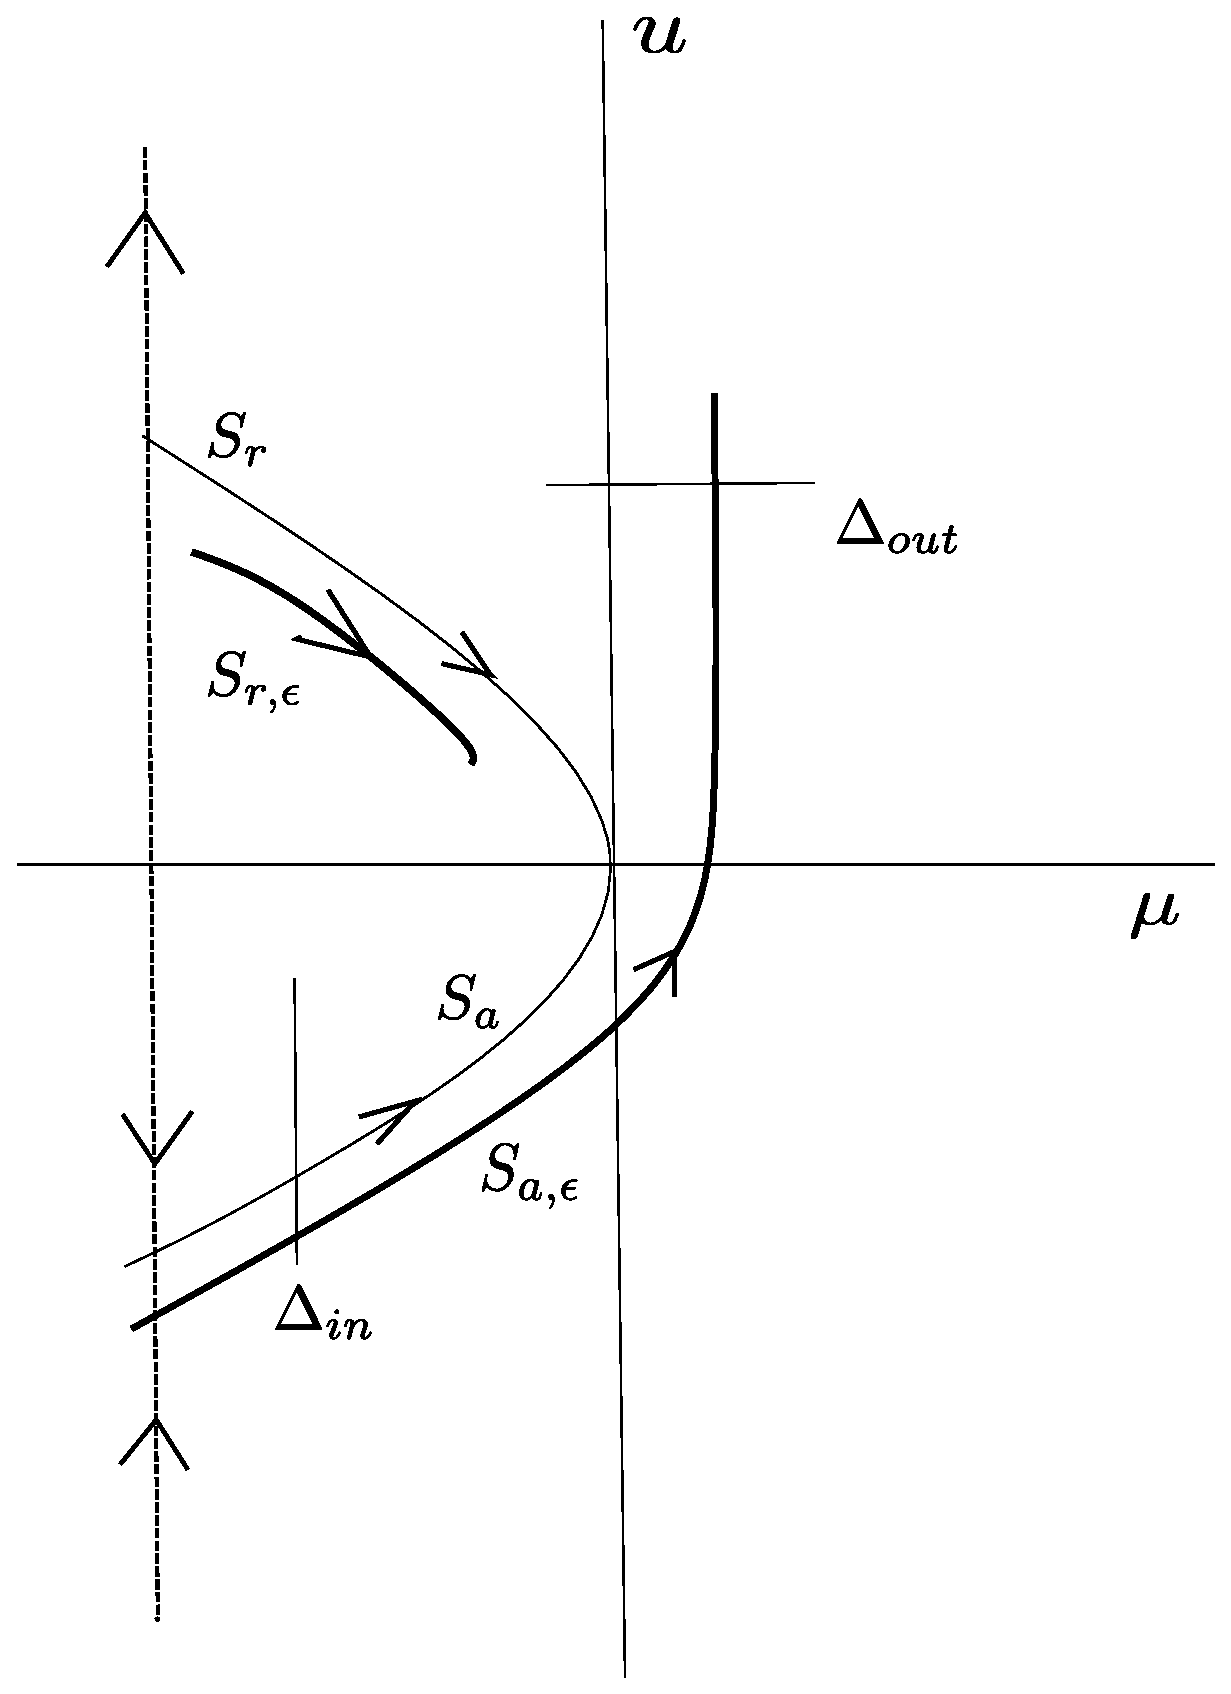
\includegraphics{pictures/passage_fold.eps}} % importing figure
 \caption{critical manifold and slow manifolds, section near the fold}\label{fig:passage}
\end{figure}

 Away from the fold point $(0,0,0)$, there exist the attracting manifold $M_a$ with a section $S_a$ sketched in Figure \ref{fig:passage}. By standard Fenichel's theory, $S_a$ perturbs to $S_{a,\eps}$ until it reaches the fold point, thus a natural question is to track how a trajectory starting on the slow manifold $S_{a,\eps}$ passes through the fold point.

Krupa and Szmolyan starts by setting two sections $\Delta_{in} = \{(-\delta, u) \mid u\in J,\text{ $J$ is some small interval }\}$ and $\Delta_{out} = \{( \mu ,\sqrt{\delta})\mid \mu \in \mathbb{R})\}$ with $\delta>0$ small but fixed, which are also shown in figure \ref{fig:passage}. To track the passage through the fold amounts to study the transition map 
\[
\pi: \Delta_{in} \to \Delta_{out},
\]

Krupa and Szmolyan then proceeds by defining the blow up transformation
\[
u =\bar{r} \bar{u},  \quad \mu = \bar{r}^2 \bar{\mu}, \quad  \eps = \bar{r}^3 \bar{\eps},
\]
which ``blows up'' the vector field of the extended $(\mu, u, \eps)$ system near $(0,0,0)$ into a vector field on the ball $B = S^2 \times [0,\eps_0^{1/3}] \ni (\bar{u}, \bar{\mu}, \bar{\eps}, \bar{r})$ for some $\eps_0>0$ small, and further directional blow-ups to obtain charts $K_1,K_2,K_3$ which was used to describe the flows in regions near different parts of the manifold $B$. After a careful and thorough analysis, they were able to prove the following results:
\begin{theorem}\label{ks_main}
For $\eps$ sufficiently small, the following statements are true:
\begin{enumerate}
\item The manifold $S_{a,\eps} $ passes through  $\Delta_{out}$ at a point $(h(\eps), \sqrt{\delta})$ where $h(\eps) = \rmO(\eps^{2/3})$.
\item The transition map $\pi$ is a contraction with rate $\rmO(e^{-c/\eps} )$, where $c$ is a positive constant.
\end{enumerate}
\end{theorem}


In this paper, we focus on the same problem \eqref{ori_eqn} with an aim to recreate the result of Theorem \ref{ks_main} via a different, functional analytically-based approach. Instead of proceeding with the geometrically-flavored blow-up approach, we directly prove a trajectory exists with the properties claimed in Theorem \ref{ks_main} by dividing the time of passage into appropriate parts and setting up corresponding ansatz in each region, closing the arguments with carefully reformulating the existence question as a fixed-point argument.

\paragraph{Outline}
The reminder of the paper is organized as follows. In Section \ref{sec_main} we give a precise statement of our result, as well as an overview of our set ups. In Sections \ref{sec_A}, \ref{sec_B} and \ref{sec_C} we construct the ansatz mentioned earlier and in Section \ref{sec_glue} we show how to piece together all the parts to arrive at our main results.


\paragraph{Notation}
We use $A \lar B$ to indicate that there is a constant $C$ such that $A \le C \cdot B$, independent of the properties of $A$ and $B$. We also use the brackets $\langle x \rangle$ to represent the expression $\sqrt{x^2+1}$.



\section{Main Result}\label{sec_main}
We first make a change of variable to transform equation \eqref{ori_eqn} into a more convenient form in section \ref{euler_m}. Then we introduces the different ansatz used in section \ref{Ric_def} and \ref{c_mfld}. We then give a statement of our main result in Section \ref{main_sum} and in Section \ref{t_sigma} we explain how we divide up the passage time into 3 different regions $A$, $B$, and $C$ to prepare for the proof of this theorem.

\subsection{Euler multiplier}\label{euler_m}
Let $\tau$ denote the independent time variable in \eqref{ori_eqn}, since for $u,\mu,\eps$ small, $g(u,\mu,\eps) = 1 + \rmO(u,\mu,\eps)>0$, we can define a new time $t = t(\tau)$ by $\frac{dt}{d\tau} = g$, consequently, equation \eqref{ori_eqn}  is transformed into
\begin{align}\label{euler_ori_eqn}
\begin{split}
\frac{d}{dt}u &= \mu+u^2+ \tilde{f}(u,\mu;\eps),\\
\frac{d}{dt}\mu &=  \eps ,
\end{split}
\end{align}
where now $\tilde{f}(u,\mu,\eps) = \rmO(\eps,  u\mu, \mu^2,\eps u, \eps \mu, \eps u^2, u^3)$.  The critical manifold 
\[
\tilde{S}_0 = \{ (\mu, u) \mid \mu + u^2 + \tilde{f}(u,\mu;0) = 0\},
\]
still has $(0,0,0)$ as the only fold point, and our goal is to track how a trajectory of the flow of \eqref{euler_ori_eqn} passes through the fold. Following the set up of the sections $\Delta_{in}$ and $\Delta_{out}$ in Krupa-Szmolyan, we propose the following boundary conditions

\begin{equation}\label{ori_bc}
\mu(0) = -\delta, \hspace{0.2in} u(T) = \delta,
\end{equation}
where $T$ is also an unknown variable which marks the ``time of exit'' as the trajectory hits the section $\Delta_{out}$.

That is, we think the tracking of the passage of the fold as a shooting problem, if we can prove the existence of a solution $(\mu, u)$ to system \eqref{euler_ori_eqn} with the boundary condition \eqref{ori_bc}, and give the expansion for the components $\mu$, then we will prove the results in \eqref{ori_eqn}. Our contribution in this paper is that the method we used to prove the existence of such a solution is different than the blow-up approach.

In the rest of the paper, we shall drop the tilde to use $f(u,\mu,\eps)$ as the nonlinearity and $S_0$ to denote the critical manifold.



\subsection{The Riccati equation}\label{Ric_def}
First, we want to get an idea of what kinds of ansatz one should use. We start with the simple case when \eqref{ori_eqn} has $f(u,\mu;\eps) = 0$ where the equation reduces to the Riccati equation,
\begin{equation}\label{ric}
\frac{d}{ds}u(s) = s+u(s)^2,
\end{equation}

we denote any solution to \eqref{ric} as $u_R$, it is known to have a unique solution (denoted by $\bar{u}_R$) with the following asymptotic expansions:

\begin{equation} \label{ric_asy}
\bar{u}_R(s)=\begin{cases}
  (\Omega_0-s)^{-1}+\rmO(\Omega_0-s), \text{ as }s \to \Omega_0, \\
 -(-s)^{1/2} -\frac{1}{4}(-s)^{-1} + \rmO(|s|^{-3/2}), \text{ as }s \to -\infty.
\end{cases}
\end{equation}

Here the constant $\Omega_0 \approx 2.3381$ is the smallest positive zero of 
\[
J_{-1/3}(2z^{3/2}/3)+J_{1/3}(2z^{3/2}/3),
\]
where $J_{\pm 1/3}$ are Bessel functions of the first kind. (See [Krupa, Szmolyan])


More generally, we consider family of solutions  $u_R(s; u_0)$ of the Riccati equation  \eqref{ric} such that $u_R(0; u_0) = u_0$. That is, we take the initial condition $u_0$ as a parameter to the Riccati equation. For the special Riccati solution $\bar{u}_R$, we denote $\bar{u}_R(0) $ as $\bar{u}_0$. In fact, using simple phase plane analysis, we can extend the asymptotic results about the special Riccati solution $\bar{u}_R$, \eqref{ric_asy} to the $u_0$-parameter dependent family $u_R(s; u_0)$, as the following proposition states.

\begin{proposition}\label{para_ric}
There exist blow up time $\Omega_\infty = \Omega_\infty(u_0)$ that depends smoothly on $u_0$ for $|u_0 - \bar{u}_0|<\eta$, $\eta$ small, with $\Omega_\infty(\bar{u}_0) = \Omega_0$, and the corresponding solution $u_R(s; u_0)$ to the Riccati equation \eqref{ric} of the form
\begin{equation}\label{ric_exp}
u_R(s;u_0) = \frac{1}{\Omega_\infty-s} +  (\Omega_\infty-s) r(\Omega_\infty-s;u_0),
\end{equation}
where the function $r$ is smooth in both variables and satisfies
\begin{equation}\label{ric_reminder}
r( \Omega_\infty-s; u_0) = -\frac{\Omega_\infty}{3} + \rmO(\Omega_\infty-s),
\end{equation}
as $s \to \Omega_\infty$.
\end{proposition}
we postpone the proof of this proposition to the appendix.
\subsection{Critical manifold}\label{c_mfld}
Another piece of the ansatz comes from part of  the critical manifold, we expect this because away from the fold, the critical manifold has an attracting branch $S_a$ which implies trajectory has to stay close to it. 

Recall the critical manifold for system \eqref{crit_mfld} is the set of points $(\mu, u) \in \mathbb{R}^2$ which satisfies
\begin{equation} \label{crit_mfld}
\mu + u^2 + f(u,\mu; 0) =  0.
\end{equation}

By the implicit function theorem, whenever $\partial_u( u^2+f(u,\mu;0) ) \neq 0$, we may write $u=u_-(\mu),$ for some function $u_s$ with $\mu$ small. For those $(\mu, u)$ such that $\partial_u( u^2+f(u,\mu;0) )<0$ (which corresponds to the attracting branch $S_a$), we define $u_s(t):= u_-(\mu(t))$ so that
\begin{equation}\label{singular}
0 = \mu(t) + u_s^2(t)+f(u_s(t),\mu; 0),
\end{equation}
for $t$ small.  

Due to the simple form of \eqref{euler_ori_eqn} and \eqref{ori_bc}, we have that $\mu(t)= \eps t-\delta$, then it can be calculated that $u_s(\mu)$ has the following asymptotic expansions
\begin{align}\label{singularAsy}
\begin{split}
u_-(\mu) &= -\sqrt{-\mu} + \rmO(|\mu|)\\
u_s(t) &= -\sqrt{\delta-\eps t} + \rmO(|\delta-\eps t|).
\end{split}
\end{align}
Similarly, we also define the upper repelling branch $u_+(\mu)$ by implicit function theorem, where we know $u_+$ satisfies
\begin{equation}
u_+(\mu) = \sqrt{-\mu} + \rmO(|\mu|) 
\end{equation}

\subsection{Main result - summary} \label{main_sum}

We now state our main result. Recall $\mathcal{U}$ is a neighborhood small enough so that \eqref{fold_nonlinearity} holds for $(\mu, u , \eps) \in \mathcal{U}$.

\begin{theorem}\label{thm:main}
Fix $\delta>0$ and $\alpha$ with $0<\alpha <3/4$, there exist $\eps_0>0,$ a constant $C=C(\delta,\alpha),$ such that for all $0<\eps<\eps_0$ and $u_i$ with $|u_i -u_-(-\delta) | \le C\eps^{1-\alpha/3}$, a solution of the rescaled system 
\begin{equation}\label{main_eqn}
\begin{split}
\frac{d}{dt}u &= \mu+u^2+ f(u,\mu;\eps), \\
\frac{d}{dt} \mu &= \eps.  \\
\end{split}
\end{equation}
with the initial condition
\begin{equation}\label{main_ic}
\begin{split}
u(0) &= u_i, \\
\mu(0) &= -\delta,
\end{split}
\end{equation}

exists on $t \in (0,T)$, where
\begin{equation}
T = \eps^{-1}\delta + \rmO(\eps^{-1/3}),
\end{equation}

and 
\begin{equation}
 u(T) = \delta.
\end{equation}
In particular, we have 
\begin{equation}
\mu(T) = \eps T -\delta = \rmO(\eps^{2/3})
\end{equation}
\end{theorem}

To fully recover Theorem \ref{ks_main}, we have  the following corollary, which is proven using the standard Fenichel theory.
\begin{corollary}\label{cor:main}
For $\alpha,\delta>0$, there is a compact interval $K \subset (-\infty, u_+(-\delta))$, independent of $\eps$ so that for all $u_i \in K$ with $(u_i,\mu,\eps) \in \mathcal{U}$, the same conclusion of Theorem \ref{thm:main} holds. Moreover, $\mu(T)$ has the following more precise expansion in $\eps$,
\begin{equation}\label{T_exp_+}
\mu(T)  = \Omega_0\eps^{2/3} + \rmO(\eps^{1-\alpha/3}),
\end{equation}
where $\Omega_0$ is the constant in \eqref{ric_asy}.
\end{corollary}

 The proof of Theorem \ref{thm:main} and \ref{cor:main} will take up the rest of the paper,  we first prepare ourselves with the setup of the problem in the following sections.

\subsection{Division of regions and the rescale of time}\label{t_sigma}

Having introduced the form of the ansatz, the next step is to ``glue'' them together. Since these ansatz have quite different asymptotic expansions at different times, it motivates us to divide the total time of of passage, from $t=0$ to $t=T$, and to choose the particular form of the ansatz, as follows:

Going backwards in time, we start with the exit time $t=T$ when the trajectory hits the section $\Delta_{out}$. Also, we use $T$ to mark the rightmost boundary of the region $A$, where our proposed solution takes the form
\[
u_A(t; u_0) = u_*(t;u_0)  + w_r(t;u_0),
\]
here the function $u_* = u_*(t; u_0)$ is defined as:
\begin{equation}\label{urdef}
u_*(t; u_0) := \eps^{1/3}u_R(\eps^{1/3}(t-\eps^{-1}\delta); u_0),
\end{equation}
where $u_R=u_R(s; u_0)$ is the family of solutions to the Riccati equation which were shown to exist in proposition \ref{para_ric}, it solves the initial value problem
\begin{equation}\label{ureq}
\frac{d}{dt}u_*(t; u_0) = \mu(t) + u_*^2(t; u_0), \hspace{0.2in} u_*(\eps^{-1}\delta; u_0) = \eps^{\frac{1}{3}} u_0,
\end{equation}
with $\eps$ and $u_0$ as parameters.  The function $w_r$ is a correction term whose properties will be given in later sections. 

In region $A$, the ansatz $u_*(t)$ is merely a rescaled version of the Riccati solution $u_R(s; u_0)$, which follows the first half of the asymptotic expansion in Proposition \ref{para_ric}. When $u_*(t)$ start to be controlled by the other part of the asymptotic expansion, we will need to adaptively change our ansatz or function space in order to ``glue'' the solutions, an intuitive, but rather arbitrary place to switch regions is at $t = \eps^{-1} \delta$. This marks the start of region $B$, where our choice of solution is as follows:
 \[ 
 u_B(t) = \bar{u}_*(t)  +w_\ell(t).
\]

Where $\bar{u}_*$ is the function
\begin{equation}\label{uldef}
\bar{u}_*(t) = u_*(t;\bar{u}_0) = \eps^{1/3} u_R( \eps^{1/3}(t-\eps^{-1}\delta); \bar{u}_0)=\eps^{1/3}\bar{u}_R(\eps^{1/3}(t-\eps^{-1}\delta)),
\end{equation}
and $\bar{u}_*$ solves the equation
\begin{equation}\label{uleq}
\frac{d}{dt}\bar{u}_* (t) = \mu(t) + \bar{u}_*^2(t),
\end{equation}
so similarly $\bar{u}_*$ is a rescaled version of the special solution to the Riccati equation. Also similar to the situation in region $A$, $w_\ell$ is a correction term whose properties will be described later.

The next piece of the ansatz will be used to connect the piece $u_B$, which roughly follows the special Riccati solution $\bar{u}_R$, to the attracting branch $S_a$ of the critical manifold $S_0$, a natural ``gluing point'' is at where the error between $\bar{u}_R$ and $u_s(t)$, is small. Calculation shows that this is at a point $t=t^*$ where we roughly have
\begin{equation}
(\delta - \eps t^*) \approx -\eps^{1/2},
\end{equation} 

hence we choose $t^*$ as a natural transition point from region $B$ to the last region, region $C$, where it covers the rest of the passage time until at $t=0$. The corresponding solution will take the form
\[
u_C(t) = u_s(t) + w_s(t),
\]
the $w_s(t)$ is yet another correction term whose properties will be discussed later. 

In summary, region $A$, $B$ and $C$ are divided as follows:
\begin{align}\label{region_division_t}
\begin{split}
\text{Region A:} & \quad (\eps^{-1}\delta, T), \quad \text{solution in region A:} \quad u_A(t) = u_*(t)+w_r(t), \\
\text{Region B:} & \quad (t^*, \eps^{-1}\delta), \quad \text{solution in region B:} \quad u_B(t) = \bar{u}_*(t)+w_\ell(t),  \\
\text{Region C:} & \quad (0, t^*), \quad \text{solution in region C:} \quad u_A(t) = u_*(t)+w_s(t), .
\end{split}
\end{align}

Now we can briefly describe the strategy of our proof, we plug in the ansatz into Equation \eqref{euler_ori_eqn} to derive the equation for the ansatz $w_r, w_\ell $ and $w_s$, choose appropriate function space with norms and set up the equations for ansatz as fixed point argument on these function spaces. A main technical part of our proof consists of appropriately rescale the time $t \in (0,T)$ so that we gain hyperbolicity in the sense that the linearized operator at the ansatz become Fredholm in the new time scale. This is the key observation in our approach, comparable to the blow-up approach which also gains hyperbolicity via a carefully chosen change of variable. Having solved the correction term $w_r, w_\ell$ and $w_s$, we can then collect information about their asymptotic expansion to confirm the corresponding solution has the properties we need.


Therefore, we need to describe how we transform time $t$ into time $\sigma$ to gain hyperbolicity. This is demonstrated in the following steps.
\begin{enumerate}
\item Step 1: Define $\psi$ as
\[
\psi = \eps^{1/3}(t - \eps^{-1}\delta),
\]

\item Step 2:
Fix $M>0$ large, define $\sigma$ as
\begin{equation} \label{psi_def}
\psi = \psi(\sigma; u_0) =\begin{cases}
-(-\frac{3}{2} \sigma)^{2/3} , &\text{ for }\sigma \le -M, \\
\Omega_\infty(u_0) -e^{-\sigma}, &\text{ for }\sigma \ge M,
\end{cases}
\end{equation}

here $\Omega_\infty$ is the blow-up time for $u_R$ found in proposition \ref{para_ric}.

Also, we denote $\varphi(\sigma) := \frac{d}{d\sigma}\psi(\sigma)$, which has the following asymptotic expansions: 
\begin{equation} \label{phi_def}
\varphi(\sigma)  =\begin{cases}
(-\frac{3}{2} \sigma)^{-1/3} , &\text{ for }\sigma \le -M, \\
e^{-\sigma}, &\text{ for }\sigma \ge M,
\end{cases}
\end{equation}
\item Step 3: For $\sigma \in (-M, M)$, we define $\psi(\sigma)$ as the straight line connecting the two points $(M, \Omega_\infty-e^{-M})$ and $(-M, -(\frac{3}{2}M)^{2/3})$. As a result, if we define $\sigma_m=\sigma_m(u_0)$ as the value of $\sigma$ such that $\psi(\sigma_m; u_0) = 0$, then we have 
\[
\frac{|\sigma_m - M|}{M} = \left| \frac{(\frac{3M}{2})^{2/3}-(\Omega_\infty-e^{-M})}{(\frac{3M}{2})^{2/3}-(\Omega_\infty+e^{-M})} -1 \right|\le CM^{-2/3},
\] 
for some constant $C$ independent of $u_0$.

Therefore we can write
\begin{equation}\label{sigm_asy}
\sigma_m = M + M_r, \hspace{0.2in} |M_r| \le CM^{1/3}.
\end{equation}
\end{enumerate}

After defining the time transformation, the original exit time $t=T$ will be transformed into $\sigma=\sigma_T$ under this change of variable, and similarly the boundary between region $A$ and region $B$ is  transformed from $t=\eps^{-1}\delta$ to $\sigma = \sigma_m$ and the boundary between region $B$ and region $C$ is  transformed from $t=t^*$ to $\sigma = \sigma^*$, and $t=0$ into $\sigma = \sigma_0$. We will see later that the $\sigma_0, \sigma^*, \sigma_m, \sigma_T$ satisfies:
\[
\sigma _0 \approx -\delta^{3/2}\eps^{-1}, \quad \sigma ^* \approx -\eps^{-1/4}, \quad \sigma_m = \rmO_\eps(1), \quad
\sigma_T \approx -\log(\eps^{1/3}\delta^{-1}) 
\]
In summary, the regions in time $\sigma$ are as follows:
\begin{align}\label{region_division_sig}
\begin{split}
\text{Region A:} & \quad (\sigma_m ,\sigma_T ),  \\
\text{Region B:} & \quad (\sigma^*, \sigma_m),  \\
\text{Region C:} & \quad (\sigma_0, \sigma^*),
\end{split}
\end{align}
and the following picture summarizes the relationship between the two time scales $t$ and $\sigma$, as well as the corresponding regions divided. 

\begin{figure}[ht]
 \centering % centering figure
 \scalebox{0.6} % rescale the figure by a factor of 0.3
 {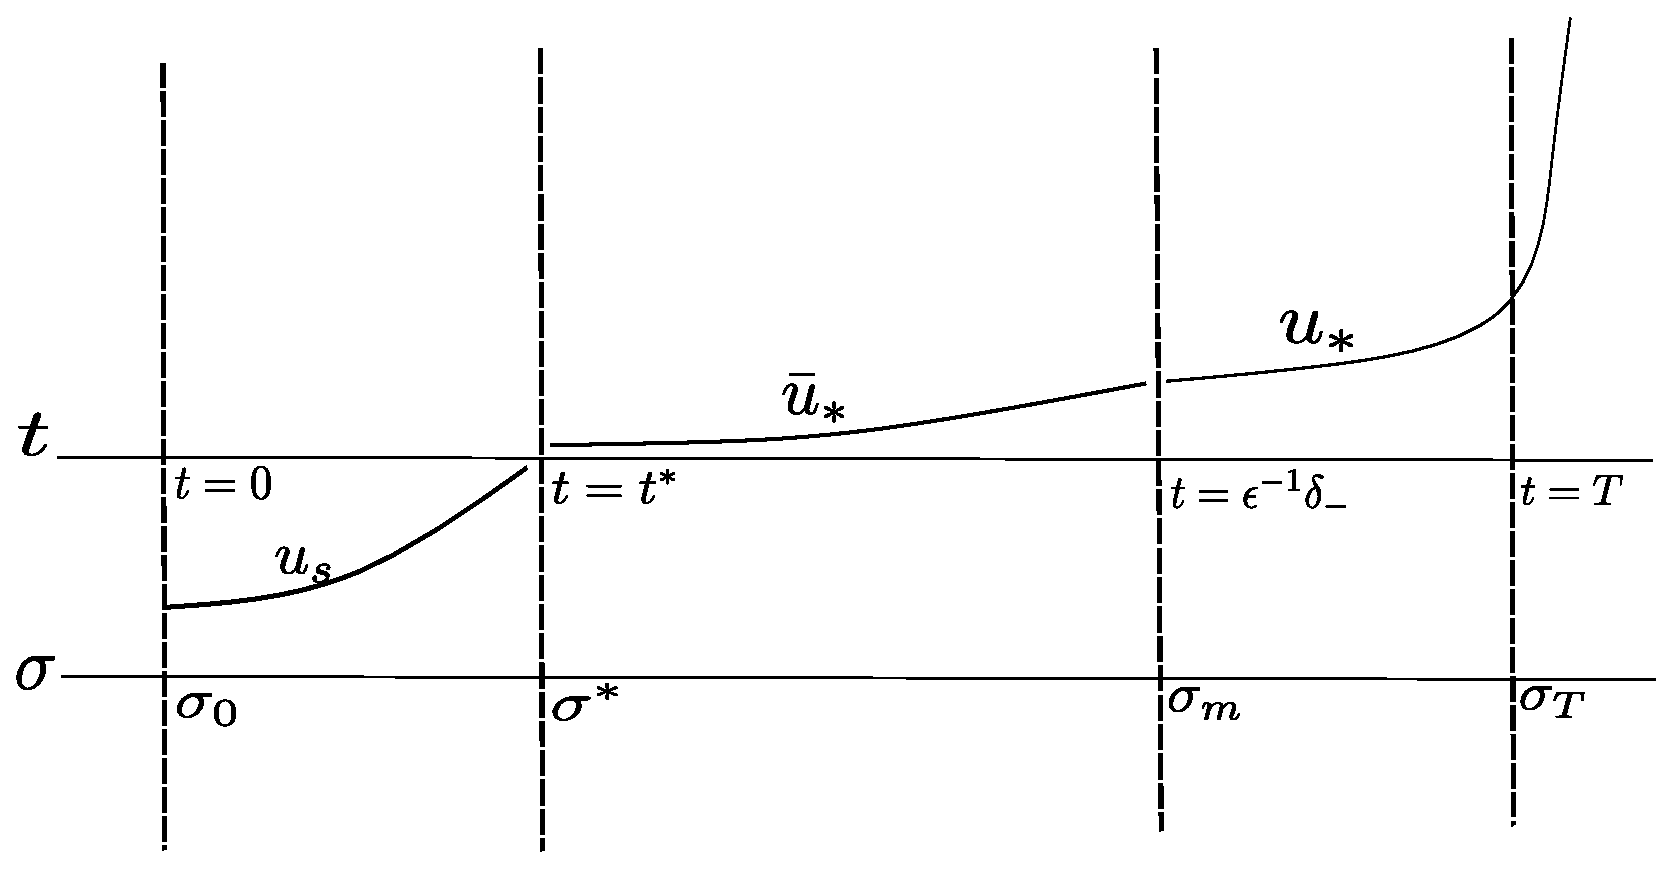
\includegraphics[angle = 0, origin = c]{pictures/time_scale.eps}} % importing figure
 % labeling to refer it inside the text
 \caption{time scales used to divide the regions}
\end{figure}\label{fig:time_scale} 

\iffalse
%\item Asymptotics for $u_R$ and $\varphi$.
\begin{equation*}
\varphi(\sigma) =\begin{cases}
 (-\frac{3}{2}\sigma)^{-1/3}, \text{ as }\sigma \to -\infty\\
e^{-\sigma} , \text{ as }\sigma \to \infty.
\end{cases}
\end{equation*}

\begin{equation*}
u_R(\psi(\sigma)) \to \begin{cases}
 -(-\frac{3}{2}\sigma)^{1/3}, \text{ as }\sigma \to -\infty\\
e^{\sigma} , \text{ as }\sigma \to \infty.
\end{cases}
\end{equation*}

\begin{equation*}
2u_R\varphi(\sigma) \to\begin{cases}
-2+ \rmO((-\sigma)^{-3/2}), \text{ as }\sigma \to -\infty\\
2+ \rmO(e^{-2\sigma}), \text{ as }\sigma \to \infty.
\end{cases}
\end{equation*}
%
\fi

\section{Region A}\label{sec_A}

Region A corresponds to the $t$-time interval $\{ t : t > \eps^{-1}\delta\}$. In this section we will give the precise form of the solution which solves system \eqref{euler_m} on this region.

\subsection{Solution in region A}

\begin{theorem}\label{thm:r}
Fix $\alpha>0, \delta>0, \eta>0$ small enough, there exists $\eps_A>0$ and a constant $C=C(\alpha,\delta,\eta)$, such that for all $0<\eps <\eps_A$, and all $|u_0 - \bar{u}_0|<\eta$, there exist a time $T=T(\eps;u_0)$, such that a solution of the form
\begin{equation}
u_A(t;u_0) = u_*(t; u_0) + w_r(t; u_0),
\end{equation}
to the rescaled system \eqref{main_eqn} exists on the time interval $t \in (\eps^{-1}\delta, T)$,
where
\begin{equation}
u_*(t; u_0) = \eps^{1/3}u_R(\eps^{1/3}(t-\eps^{-1}\delta); u_0),
\end{equation} and $u_R(\cdot; u_0)$ is the family of solution to Riccati equation that were shown to exist in Proposition \ref{para_ric}. 

Moreover, we have
\begin{enumerate}[label=\textnormal{(\arabic*)}]
\item \label{thm:r_1}$T=T(\eps;u_0) = \eps^{-1}\delta+\eps^{-1/3}\Omega_\infty(u_0)-\delta^{-1}+T_r$ with $T_r = \rmO( \eps^{2/3}\delta^{-3} )$ where the constant $\Omega_\infty(u_0)$ is the same mentioned in Proposition \ref{para_ric},
\item \label{thm:r_2} $w_r(T; u_0) = 0$ and $u_*(T,u_0)=\delta$,
\item \label{thm:r_3} $w_r$ is continuous with $|w_r(\eps^{-1}\delta; u_0)| \le C\eps^{(2-\alpha)/3}$.

\item \label{thm:r_4} $ |w_r(t; u_0)| \le C|T_\infty-t|^{\alpha-2}$ for $t \in (\eps^{-1}\delta, T)$.

\item \label{thm:r_5} The function 
$\mathcal{F}: (\bar{u}_0-\eta, \bar{u}_0+\eta) \to \mathbb{R}$ with $\mathcal{F}(u_0)=  w_r(\eps^{-1}\delta; u_0)$ is smooth, with Lipschitz constant satisfy 
\[
|\text{Lip }\mathcal{F} |\le C\eps^{2/3} . 
\]
\end{enumerate}

\end{theorem}

We will prove this theorem in the following sections.
\subsection{The exit time \texorpdfstring{$T(u_0)$}{T(u_0)}}\label{exit_time}
Take $\eta>0$ so that the function $u_R = u_R(\cdot; u_0)$ exists for $|u_0-\bar{u}_0|<\eta$ as demonstrated in Proposition \ref{para_ric}. The exit time $T$ is then defined by the condition 
\[
\delta = u_*(T; u_0) = \eps^{1/3}u_R(\eps^{1/3}(T-\eps^{-1}\delta); u_0),
\]
since the expansion for $u_R$ is given in \eqref{ric_exp} , if we define $\psi_T = \eps^{1/3}(T-\eps^{-1}\delta)$, then $\psi_T$ satisfies
\[
\frac{1}{\Omega_\infty-\psi_T} + (\Omega_\infty-\psi_T)r(\Omega_\infty-\psi_T) = \eps^{-1/3}\delta,
\]
from which we get the leading order expansion $\Omega_\infty-\psi_T = \rmO(\eps^{1/3}\delta^{-1})$. A fixed point argument gives
\[
\Omega_\infty - \psi_T = \eps^{1/3}\delta^{-1} + \rmO(\eps \delta^{-3}),
\]
hence the expansion for $T=T(\eps; u_0)$ is
\begin{equation}\label{T_exp}
T = T(\eps;u_0) = \eps^{-1}\delta + \eps^{-1/3}\Omega_\infty(u_0) - \delta^{-1} + T_r,
\end{equation}
with 
$|T_r|\le C\eps^{2/3}\delta^{-3}$, for some constant $C$ independent of $u_0$, as $\eps \to 0$.

For convenience, we define \[
T_\infty = T_\infty(\eps; u_0)= \eps^{-1}\delta + \eps^{-1/3}\Omega_\infty(u_0),
\]
so that $T = T_\infty - \delta^{-1} + T_r$.

\subsection{Equation for \texorpdfstring{$w_r$}{wr} and rescaling}\label{equation_wr}
We now plug in $u = u_* + w_r$ into equation \eqref{euler_m}, and derive the equation for $w_r$
\begin{align}\label{eqn_wr}
\begin{split}
w_r' - 2u_*w_r &= w_r^2 + f(u_*+w_r, \mu; \eps) := R_r(w_r; \eps,u_0),
\end{split}
\end{align}

moreover, we enforce the boundary condition $u(T; u_0) = \delta$, hence this gives the boundary condition for $w_r$ at $t=T$:
\begin{equation}\label{Bc_w_r}
w_r(T;u_0) = 0,
\end{equation}


therefore, we need to solve equation \eqref{eqn_wr} on the interval $t \in (\eps^{-1}\delta, T)$, with boundary condition \eqref{Bc_w_r}.

Next, we rescale equation \eqref{eqn_wr} into $\sigma$-time variable by using the $t$ to $\sigma$-time rescaling in section \ref{t_sigma}, and obtain
\begin{equation}\label{rescl_wr}
\left(\frac{d}{d\sigma} - a(\sigma; \eps, u_0)\right) W_r =\eps^{-1/3}\varphi \mathcal{R}_r(W_r; \eps,u_0),
\end{equation}
where
\begin{itemize}
\item The term $a(\sigma;\eps, u_0)$ is defined as and has asymptotic expansion
\[
a(\sigma; \eps, u_0) := 2\varphi(\sigma)u_R(\psi(\sigma); u_0) =  2+\rmO(e^{-2\sigma}) \text{ as }\sigma \to \infty,
\]
we remark that this convergence as $\sigma \to \infty$ is uniform in $u_0$ due to the definition of our time-rescaling.

\item The function $W_r(\sigma)$ is the rescaled version of $w_r(t)$ in the $\sigma$-variable, $w_r(t) = w_r(\eps^{-1/3}\psi(\sigma)+\eps^{-1}\delta) = W_r(\sigma)$. $U_*$ is similarly the rescaled version of $u_*$,  $U_*(\sigma;u_0)= u_*(t;u_0) = \eps^{1/3}u_R(\psi(\sigma;u_0);u_0)$.

\item The function $\Ral_r$ is a rescaled version of $R_r$ such that 
\[
\mathcal{R}_r(W_r;\eps,u_0) = W_r^2 + f(U_*+W_r, \mu ; \eps),
\]
\end{itemize}
 

To get the corresponding boundary condition of \ref{Bc_w_r}, we need to know the corresponding $\sigma$-time for the $t$-time interval $t\in (\eps^{-1}\delta, T)$.

At $t = \eps^{-1}\delta$, the corresponding $\sigma$ time is at $\sigma=\sigma_m$, from its definition in section \ref{t_sigma}.

At $t=T$, we have $\eps^{1/3}(T-\eps^{-1}\delta) = \Omega_\infty -\eps^{1/3}\delta^{-1}+\eps^{1/3}T_r=\psi(\sigma_T) = \Omega_\infty-e^{-\sigma_T}$ from \eqref{T_exp}, hence, for $\eps$ small enough, we get that the corresponding $\sigma$-time to $t=T$ is 
\begin{equation}\label{def_sigm_T}
\sigma_T=\sigma_T(u_0)= -\log(\eps^{1/3}(\delta^{-1}-T_r)) = -\log(\eps^{1/3}\delta^{-1}) - \log(1-\delta T_r),
\end{equation}
then, the complete boundary value problem we wish to solve is
\begin{align}\label{wr_bp}
\begin{split}
\frac{d}{d\sigma} W_r - a(\sigma;\eps,u_0)W_r &= \eps^{-1/3}\varphi \Ral_r(W_r), \text{ for } \sigma \in (\sigma_m, \sigma_T),\\
W_r(\sigma_T) &= 0.
\end{split}
\end{align}




\subsection{Linear equation and norms}




Our goal now is to solve \eqref{wr_bp} on an appropriate function space, to do so we first slightly enlarge the time interval $(\sigma_m, \sigma_T)$ where the boundary value problem is posed.

From the definition of $\sigma_T$ \eqref{def_sigm_T}, we see that
\begin{equation}\label{sigm_T_asy}
|\sigma_T -(-\log(\eps^{1/3}\delta^{-1}))| \le |\log(1-\delta T_r)| \le  C|\delta T_r|\le C\eps^{2/3}\delta^{-2},
\end{equation} 
for some constant $C$ independent of those $u_0$ with $|u_0-\bar{u}_0|<\eta$.

We now define $\sigma_{\inf}$ and $\sigma_{\sup}$ as follows:
\[
\sigma_{\inf} = \inf_{|u_0-\bar{u}_0|<\eta}\sigma_m(u_0), \hspace{0.3in} \sigma_{\sup} = \sup_{|u_0-\bar{u}_0|<\eta}\sigma_T(u_0).
\]
From the definition of $\sigma_m$ in section \ref{t_sigma} and \eqref{sigm_T_asy} we have
\[
M \approx\sigma_{\inf} , \hspace{0.2in} \sigma_{\sup} \approx -\log(\eps^{1/3}\delta^{-1}),
\] with the error independent of $u_0$. 
Therefore we introduce the following weighted function space:
\begin{align*}
\mathcal{C}_{r} &= \left\{ w(\sigma) : \sup_{\sigma_{\sup}\ge \sigma\ge \sigma_{\inf}} \left|\eps^{(\alpha-2)/3} e^{(\alpha-2)\sigma}w(\sigma)\right| < \infty \right\}. \\
%--------------------------------------
\end{align*}

We establish the invertibility of the linear operator $A_r$ which acts on $w \in \mathcal{C}_r$ as 
\[
A_r w = \left( \frac{d}{d\sigma}w-a(\sigma;\eps, u_0) w,  w(\sigma_T)\right),
\]
in the following
\begin{proposition}\label{inv_A_r}
$A_r=A_r(u_0,\eps) : \mathcal{D}\subset \mathcal{C}_r \to \mathcal{C}_r\times \mathbb{R}$ and is invertible, with its inverse  depends smoothly and uniformly bounded in $u_0, \eps$. 
\end{proposition}
\begin{proof}
Consider the conjugate operator of $A_r$, given by
\begin{align*}
\tilde{A}_r v &= \left( e^{(\alpha-2)\sigma}\left(\frac{d}{d\sigma}-a(\sigma;\eps,u_0)\right)e^{(2-\alpha)\sigma} v, v(\sigma_T) \right) \\
&= \left( \frac{d}{d\sigma}v -(\alpha+a(\sigma;\eps,u_0)-2)v, v(\sigma_T) \right),
\end{align*}
for $v(\sigma)=\eps^{(\alpha-2)/3}e^{(\alpha-2)\sigma}w(\sigma) \in \mathcal{C}(\sigma_{\inf}, \sigma_{\sup})$. 

The associated conjugate equation of 
\[
A_r w = (f,w_T) \text{ with } f \in \mathcal{C}_r, w_T \in \mathbb{R},
\] is 
\[
\tilde{A}_r v = (\eps^{(\alpha-2)/3}e^{(\alpha-2)\sigma} f,v_T) \text{ with } \eps^{(\alpha-2)/3}e^{(\alpha-2)\sigma} f \in C , v_T = \eps^{(\alpha-2)/3} e^{(\alpha-2)\sigma_T}w_T.
\]
 
Since $\alpha > 0$ and $|a(\sigma;\eps,u_0) -2| = \rmO(e^{-2\sigma}) \to 0$ as $\sigma \to \infty$ uniformly in $\eps, u_0$. We apply lemma \ref{lin_bv} with $L= \sigma_T$ to conclude that there exists a constant $C$ independent of $\eps, u_0$ with 
\[
\|w\|_{\mathcal{C}_r} = |v|_\infty \le C(|\eps^{(\alpha-2)/3}e^{(\alpha-2)\sigma} f |_{\infty}+|v_T|) \le C(\|f\|_{\mathcal{C}_r}+|w_T|),
\]
notice $|v_T| \le w_T$ by the asymptotic expansion of $\sigma_T  = \rmO(-\log(\eps^{1/3}))$. By the definition of $\sigma_{\inf}$ and $\sigma_{\sup}$, $A_r$ is uniformly invertible in $u_0$ on $\mathcal{C}_r$, this finishes the proof of the proposition.
\end{proof}

\iffalse
\begin{proof}
Fix $\eta$ small, then there is $\eps_0>0$ such that for $\eps<\eps_0$, we can choose $\sigma_* \in (\sigma_{\inf}, \sigma_{\sup})$ so that $|a(\sigma; \eps, u_0)-2| \le \eta$ for $\sigma \ge \sigma_*$. As a result there is a constant $C$, independent of $\eps$ and $u_0$, such that $|\sigma_*-\sigma_{\inf}|\le C$. In fact, we can choose $\sigma_* \le \sigma_T$ since $|\sigma_T-\sigma_{\sup}| \le |\sigma_T - (-\log(\eps^{1/3}\delta^{-1})|\le C\eps^{2/3}\delta^{-2}$.

For $\sigma_{\sup} \ge \sigma \ge \sigma_*$, the linear operator $A_r$ is a small perturbation of the invertible linear operator $w \to \left(\frac{dw}{d\sigma}-2w, w(\sigma_T) \right)$. Indeed, for $f \in \mathcal{C}_r$, the equation $\frac{d}{d\sigma}w-2w = f$
has the solution
\[
w(\sigma) = e^{2(\sigma-\sigma_T)}w(\sigma_T)+\int_{\sigma_T}^\sigma e^{2(\sigma-s)}f(s)ds,
\]
moreover, it holds that $\|w\|_{\mathcal{C}_r} \le C(\delta^{\alpha-2}|w(\sigma_T)| + 2\alpha^{-1}\|f\|_{\mathcal{C}_r})$ for some constant $C$ independent of $u_0,\eps$, which shows the inverse is independent of $\eps$ and $u_0$. If the prescribed value at $w(\sigma_T)$ is of order $\delta^{2-\alpha}$.

For $\sigma < \sigma_*$, we can directly write down the solution of $(d/d\sigma - a)w = f$ as
\[
w(\sigma) = \exp\left(\int^{\sigma}_{\sigma_*} a(\tau)d\tau\right) w(\sigma_*) + \int_{\sigma_*}^{\sigma} \exp\left(-\int_{\sigma}^{s}a(\tau)d\tau\right)f(s)ds 
\]
 Again, the inverse is bounded uniformly in $\eps, u_0$ because of the bound $|\sigma_*-\sigma_{\inf}|\le C$. To see this, note $w(\sigma_*)$ can be evaluated using the solution on the interval $(\sigma_*,\sigma_{\sup})$, which satisfies $w(\sigma_*) \lar \eps^{\frac{2-\alpha}{3}}e^{(2-\alpha)\sigma_*}$, so 
\[
\left\|\exp\left(\int^{\sigma}_{\sigma_*} a(\tau)d\tau\right) w(\sigma_*)\right\|_{\mathcal{C}_r} \le e^{(2-\alpha)(\sigma_*-\sigma)}\exp\left(\int^{\sigma}_{\sigma_*} a(\tau)d\tau\right) \lar e^{(2-\alpha)C},
\]
and
\[
\left\| \int_{\sigma_*}^{\sigma} \exp\left(-\int_{\sigma}^{s}a(\tau)d\tau\right)f(s)ds\right\|_{\mathcal{C}_r} \le \int_{\sigma_*}^{\sigma} \exp\left(-\int_{\sigma}^{s}a(\tau)d\tau\right)e^{(2-\alpha)(s-\sigma)} \|f\|_{\mathcal{C}_r}ds \lar e^{(2-\alpha)C}\|f\|_{\mathcal{C}_r}
\]
Combining the case $\sigma< \sigma_*$ and $\sigma \ge \sigma_*$ together, we conclude that $A_r$ is uniformly invertible in $\eps$ and $u_0$ on the space $\mathcal{C}_r$.
\end{proof}
\fi

\subsection{Nonlinear estimates}

In this section we estimate the nonlinear term
\[
\mathcal{R}_r(W_r) = W_r^2 + f(U_*+W_r, \mu ; \eps),
\]
in the $\mathcal{C}_r$ norm to prove 
\begin{proposition}\label{nl_est_r}
If $W_r \in \mathcal{C}_{r}$, then $\eps^{-1/3}\varphi \mathcal{R}_r(W_r) \in \mathcal{C}_{r}$, and
\begin{align}
\|\eps^{-1/3}\varphi \mathcal{R}_r \| = \rmO(\delta^{\alpha}).
\end{align}
\end{proposition}
\begin{proof}

Proposition \ref{ric_exp} shows
\begin{align*}
U_*(\sigma;u_0) =  \eps^{\frac{1}{3}}(e^\sigma+e^{-\sigma} r(e^{-\sigma}; u_0)   ) \text{ as }\sigma \to \infty,
\end{align*}
therefore 
\[
|U_*(\sigma)| \lar \eps^{\frac{1}{3}}e^\sigma \le \eps^{1/3}e^{\sigma_{\sup}} = \rmO(\delta) \text{ for all } \sigma \ge \sigma_{\inf}.
\]

From the definition of the time rescaling in section \ref{t_sigma} we have
\[
\mu = \eps t-\delta  =\eps^{2/3}\psi(\sigma) \lar \eps^{2/3},
\]
for all $\sigma \ge \sigma_{\inf}$.

As $W_r \in \mathcal{C}_r$, we have 
\[
|W_r(\sigma)| \lar \eps^{\frac{2-\alpha}{3}} e^{(2-\alpha)\sigma} \ll |U_*(\sigma)|, \text{ for } \sigma \in (\sigma_{\inf}, \sigma_{\sup}).
\]

Using these facts, we have
\[
\|\eps^{-\frac{1}{3}}\varphi W_r^2\|_{\mathcal{C}_r}=\sup |\eps^{-\frac{1}{3}} \varphi W_r| \lar \eps^{\frac{1-\alpha}{3}} e^{(1-\alpha)\sigma} \lar \eps^{\frac{1-\alpha}{3}} e^{(1-\alpha)\sigma_{\sup}} \lar \delta^{1-\alpha},
\]

as $f(u,\mu; \eps) = \rmO(\eps(1+u+\mu+u^2),u\mu,\mu^2,u^3)$ and since $U_*,W_r,\mu$ are all small in sup norm, we have

\[
f(U_*+W_r, \mu ;\eps) = \rmO(\eps, (U_*+W_r)\mu, \mu^2, (U_*+W_r)^3 ) = \rmO(\eps, U_*\mu, \mu^2, U_*^3),
\]

hence
\[
\|\eps^{-\frac{1}{3}}\varphi \eps \|_{\mathcal{C}_r}=\sup |\eps^{-\frac{1}{3}} \varphi  \cdot \eps \cdot \eps^{(\alpha-2)/3}e^{(\alpha-2)\sigma}| \lar \eps^{\alpha/3} e^{(\alpha-3)\sigma_m} = \rmO(\eps^{\alpha/3}) ,
\]

\[
\|\eps^{-\frac{1}{3}}\varphi U_*\mu \|_{\mathcal{C}_r} =\sup |\eps^{-\frac{1}{3}} \varphi \cdot U_*\mu \cdot \eps^{(\alpha-2)/3}e^{(\alpha-2)\sigma} | \lar \eps^{\alpha/3} e^{(\alpha-2)\sigma_m}  =\rmO( \eps^{\alpha/3}) ,
\]

\[
\|\eps^{-\frac{1}{3}}\varphi \mu^2 \|_{\mathcal{C}_r} \lar \|\eps^{-\frac{1}{3}}\varphi \eps \|_{\mathcal{C}_r} \text{ since } \mu^2 = \rmO(\eps^{4/3}) \ll \eps, 
\]
and lastly
\[
\|\eps^{-\frac{1}{3}}\varphi U_*^3\|_{\mathcal{C}_r} \lar \eps^{\frac{\alpha}{3}} e^{\alpha\sigma} \lar \eps^{\frac{\alpha}{3}} e^{\alpha\sigma_{\sup}} = \rmO(\delta^\alpha).
\]
Combining all the estimates we conclude that 
\[
\|\eps^{-1/3}\varphi \Ral_r(W_r) \| = \max\{ \rmO(\delta^\alpha), \rmO(\delta^{1-\alpha})\},
\]
since we assumed $\alpha \ll 1$, it follows that $\|\eps^{-1/3}\varphi \Ral_r(W_r) \| = \rmO(\delta^\alpha)$, this completes the proof.
\end{proof}

\subsection{Fixed point argument and the proof of Theorem \ref{thm:r}}
In this section we prove theorem \ref{thm:r} by setting up an appropriate fixed point argument.
\begin{proof}[Proof of theorem \ref{thm:r}]
Items \ref{thm:r_1} and \ref{thm:r_2} in the assertion of the theorem has been demonstrated in section \ref{exit_time} and \ref{equation_wr}. Items \ref{thm:r_3} and \ref{thm:r_4} is a direct consequence of the fact that $W_r \in \mathcal{C}_r$, to prove this, we first rewrite equation \eqref{rescl_wr} and the boundary condition $W_r(\sigma_T)=w_T$ as 
\[
F_r(W_r, w_T; \eps, u_0) = 0,
\]
where $F_r : \mathcal{C}_r\times \mathbb{R} \to \mathcal{C}_r\times \mathbb{R}$ is defined as
\begin{align*}
F_r(W_r,w_T;\eps,u_0) &= A_rW_r - \left(\eps^{-1/3}\varphi \Ral_r(W_r), w_T \right)\\
&=\left( \frac{d}{d\sigma}W_r-aW_r - \eps^{-1/3}\varphi \Ral_r(W_r), W_r(\sigma_T)-w_T \right).
\end{align*} 
%Now we are ready to use a fixed point argument to solve the equation 
%\[
%A_r W_r = (\eps^{-1/3}\varphi \mathcal{R}_r(W_r), w_T).
%\]


Let $X = \mathcal{C}_r \times I$, where $I$ is some small interval containing $0$, we introduce the solution map $\mathcal{S}: X \to \mathcal{C}_r\times \mathbb{R}$ as follows:
\[
\mathcal{S}(W_r,w_T; \eps, u_0) = (W_r-A_r^{-1}F_r(W_r,w_T;\eps, u_0), w_T),
\]

From propositions \ref{inv_A_r} and \ref{nl_est_r}, we conclude 
\begin{itemize}
\item $\|\mathcal{S}(0,0;\eps,u_0) \|= \|\left( -A_r^{-1}F_r(0,0;\eps,u_0),0\right)\| \le \|A_r^{-1}\|\|F_r(0,0;\eps,u_0)\| \lar |\|\eps^{-1/3}\varphi \Ral_r(0)\| \lar \delta^\alpha$, uniformly in $\eps$ and $u_0$.

\item $\mathcal{S}$ is a smooth map in $W_r,w_T$ as well as the parameters $\eps, u_0$.

\item Since the derivative of $f(U_*+W_r,\mu;\eps)$ with respect to $W_r$ is $D_{W_r} f(U_*+W_r,\mu;\eps)=\rmO(\mu, U_*^2)$, the linearization of $\mathcal{S}$ at $(0,0)$, $D_{(W_r,w^*)} \mathcal{S}(0,0)$ satisfies
\[
\|D_{(W_r,w^*)} \mathcal{S}(0,0)\|_{op} \lar \sup|\eps^{-1/3}\varphi(\mu+U_*^2)| = \rmO(\delta),
\]
where $\|\cdot\|_{op}$ denotes the operator norm of the associated linear operator.
Moreover, for $\|W_r\|$ small enough and $|w_T|\le \delta_1$, we have $D_{(W_r,w_T)}\mathcal{S}(W_r,w_T;\eps,u_0) =  D_{(0,0)}\mathcal{S}(W_r,w_T;\eps,u_0)+\rmO(\|W_r\|_{\mathcal{C}_r})$, which is uniformly small in $\eps$ and $u_0$.

\end{itemize}

Therefore, for $(W_r,w_T)$ in a small ball of $X$, we can apply an iteration scheme and utilize the Banach fix point theorem to the existence of a fixed point, hence a solution to equation \eqref{rescl_wr} exists. Moreover, this solution depends smoothly on the parameter $\eps, u_0$. By picking $w_T = 0$, we have shown that a unique fixed point $W_r \in \mathcal{C}_r$ exists and solves equation \eqref{rescl_wr}.


Finally, to prove item \ref{thm:r_5} we need to estimate the Lipschitz constant for the map 
\[
\Psi : u_0 \mapsto w_r(\eps^{-1}\delta; u_0)=W_r(\sigma_m;u_0),
\]
 which maps from a small interval $I$ containing $\bar{u}_0$ to $\mathbb{R}$. We can write $\Psi$ as the composition of two maps $\Psi = \Psi_1 \circ \Psi_2$ where $\Psi_2 : I \to \mathcal{C}_r$ is the map 
\[
 u_0 \mapsto W_r(\sigma; u_0),
\] 
and $\Psi_1 : \mathcal{C}_r \to \mathbb{R}$ is the evaluation map
\[
  W_r(\sigma; u_0) \mapsto W_r(\sigma_m, u_0).
\]
 
To estimate the number $\text{Lip}_{u_0} \Psi$, we need to estimate the number $\text{Lip}_{u_0} \Psi_2$ and $\text{Lip } \Psi_1$.

To estimate $\text{Lip}_{u_0} \Psi_2$, it suffices to estimate the following two quantities
\[
C_1 = \text{Lip}_{W_r} \mathcal{S}, \text{ and }C_2 = \text{Lip}_{u_0} \mathcal{S},
\]
because $W_r$ is the fixed point of the map $\mathcal{S}$, which implies
\[
\text{Lip}_{u_0} \Psi_2 \le  C_2/(1-C_1).
\]

From the definition of $\mathcal{S}$, we see that
\[
C_1 \le \text{Lip}_{W_r} |\eps^{-1/3}\varphi R_r(W_r)|\le \text{Lip}_{W_r} |\eps^{-1/3}\varphi W_r^2| \le\sup_{W_r \in \mathcal{C}_r} |\eps^{-1/3}\varphi W_r | = \rmO(\delta^{1-\alpha}),
\]
where the last line follows from proposition \ref{nl_est_r}.


To estimate $C_2$. We notice that 
\[
C_2 \le \text{ Lip }_{u_0} |\eps^{-1/3}\varphi U_*^3(\sigma;u_0) |.
\]
However if $u_0, \tilde{u}_0$ are two different numbers near $\bar{u}_0$,
\[
\|\eps^{-1/3}\varphi [U_*^3(\sigma;u_0)-U_*^3(\sigma;\tilde{u}_0)] \|_{\mathcal{C}_r} \le \|\eps^{-1/3}\varphi U_*^2 \|_{\mathcal{C}_r} \sup|U_*(\sigma;u_0)-U_*(\sigma;\tilde{u}_0)|,
\] 

proposition \ref{ric_exp} shows
$U_*(\sigma;u_0)= \eps^{1/3}(e^\sigma + e^{-\sigma} r(e^{-\sigma}; u_0))$ for $\sigma$ large, hence 
\[
\partial_{u_0} U_*(\sigma;u_0) \le C\eps^{1/3},
\]
for some constant independent of $u_0$, on the other hand
\[
\|\eps^{-1/3}\varphi U_*^2 \|_{\mathcal{C}_r}  = \rmO(\eps^{(\alpha-1)/3}),
\]
so we conclude that
\[
\|\eps^{-1/3}\varphi [U_*^3(\sigma;u_0)-U_*^3(\sigma;\tilde{u}_0)] \|_{\mathcal{C}_r} \le C\eps^{\alpha/3}|u_0 - \tilde{u}_0|,
\]
or $C_2 = \rmO(\eps^{\alpha/3})$. Hence 
\[
\text{Lip}_{u_0} \Psi_2 = \rmO(\eps^{\alpha/3}).
\]

On the other hand, the evaluation map $\Psi_1$ is a linear map which satisfies
\[
|\Psi_1(W)-\Psi_1(\widetilde{W})| = |W(\sigma_m) -\widetilde{W}(\sigma_m) | \le\|W - \widetilde{W}\|_{\mathcal{C}_r}\eps^{(2-\alpha)/3} e^{(2-\alpha)\sigma_m} \lar \eps^{(2-\alpha)/3}\|W-\widetilde{W}\|,
\]
for $W,\widetilde{W}$ in $\mathcal{C}_r$, from the definition of its norm, therefore
\[
\text{Lip } \Psi_1 = \rmO(\eps^{(2-\alpha)/3}),
\]
combine the two estimates we conclude that 
\[
\text{Lip}_{u_0} \Psi \le \left( \text{Lip}_{u_0} \Psi_2 \right) \left( \text{Lip } \Psi_1 \right) = \rmO(\eps^{2/3}),
\] 
which completes the proof of Theorem \ref{thm:r}.
\end{proof}

\section{Region B}\label{sec_B}

Region B corresponds to the $t$-time interval $ t^*< t< \eps^{-1}\delta$. In this section, we give the precise form of the solution in this region and prove the needed properties.

\subsection{Solution in region B}

\begin{theorem}\label{thm:l}
Fix $\delta>0, \alpha>0$ small enough, there exists $\eps_B>0$ and a constant $C=C(\delta,\alpha)$ such that for all $0<\eps <\eps_B$, and $w^*$ with $|w^*| \le  C\eps^{1/2-\alpha/3}$, a solution $u_B$ of the form 
\begin{equation}
u_B(t) = \bar{u}_*(t) + w_\ell(t),
\end{equation}
to system \eqref{main_eqn} with the initial condition
\begin{equation}\label{ul_ic}
u(t^*) = \bar{u}_*(t^*) + w^*, \hspace{0.2in}\mu(t^*) = \eps t^* -\delta
\end{equation}
exists on the time interval $t \in (t^*, \eps^{-1}\delta)$, where $\bar{u}_*$ is the function defined as in \eqref{uldef}. Moreover, we have that the correction function $w_\ell$ is continuous with
\begin{equation}\label{thm:l_1}
|w_\ell(t)| \le C\eps^{(2-\alpha)/3} | \eps^{1/3}(t-\eps^{-1}\delta)+1|,
\end{equation}
for $t \in (t^*, \eps^{-1}\delta)$.
\end{theorem}

We will prove this theorem in the rest of this section.
\subsection{Equation of \texorpdfstring{$W_{\ell}$}{Well} and rescaling}

As before, we plug the ansatz into \eqref{euler_ori_eqn} to derive the equation satisfied by $w_\ell$.
\begin{align}\label{Eqn_wl}
\begin{split}
w_{\ell}' -2\bar{u}_* w_\ell &= w_\ell^2 + f(\bar{u}_*+w_\ell, \mu; \eps):=R_\ell(w_\ell,\mu;\eps).
\end{split}
\end{align}

We want to solve this equation on $t\in (t^*, \eps^{-1}\delta)$. 
Following previous steps, we next rescale the equation to the $\sigma$-time variable using the time rescaling map $\psi = \psi(\sigma; \bar{u}_0)$ and we obtain
\begin{equation}\label{rescl_wl}
\frac{d}{d\sigma} W_\ell - b(\sigma)W_\ell = \eps^{-1/3}\varphi \Ral_\ell(W_\ell,\mu,\eps),
\end{equation}

where 
\begin{itemize}
\item The equation is posed on $\sigma \in (\sigma^*, \sigma_m(\bar{u}_0))$ where $\sigma^* \approx -\eps^{-1/4}$ and $\sigma_m(\bar{u}_0) := \bar{\sigma}_m$ follows the notation used in section \ref{t_sigma}.

\item The term $b(\sigma)$ is defined and has asymptotic expansion:
\[
b(\sigma) := 2u_R(\psi(\sigma))\varphi(\sigma) = -2 + \rmO(|\sigma|^{-1}),
\]
as $\sigma \to -\infty$. Again, the convergence is uniform in $\eps$.

\item The function $W_\ell(\sigma)$ is the rescaled version of $w_\ell(t)$ in the $\sigma$-variable, $w_\ell(t) = w_\ell(\eps^{-1/3}\psi(\sigma)+\eps^{-1}\delta) = W_\ell(\sigma)$. $\bar{U}_*$ is similarly the rescaled version of $\bar{u}_*$,  $\bar{U}_*(\sigma)= \bar{u}_*(t) = \eps^{1/3}\bar{u}_R(\psi(\sigma ) )$.

\item The function $\Ral_\ell$ is a rescaled version of $R_\ell$ such that $\Ral_\ell(W_r;\eps,u_0) = W_\ell^2 + f(\bar{U}_*+W_\ell, \mu;\eps),$ 
\end{itemize}

We also need to specify the boundary value at the left end point $\sigma = \sigma^*$, the complete system we want to solve is
\begin{align}\label{wl_bp}
\begin{split}
\frac{d}{d\sigma} W_\ell - b(\sigma)W_\ell &= \eps^{-1/3}\varphi \Ral_\ell(W_\ell), \text{ }\sigma \in (\sigma^*, \bar{\sigma}_m),\\
W_\ell(\sigma^*) &= w^*.
\end{split}
\end{align}

\subsection{Linear equation and norms}

Similarly, the proof of theorem \ref{thm:l} consists of solving \eqref{rescl_wl} via a fixed point argument on the following function space:
\[
\mathcal{C}_{\ell} = \left\{ w(\sigma) : \sup_{\sigma^*<\sigma<\bar{\sigma}_m} |\eps^{(\alpha-2)/3}\langle\sigma \rangle^{-2/3} w(\sigma)|<\infty \right\}.
\]

%The homogeneous solution $u$, which solves the equation $u_\sigma = b(\sigma) u$ on the whole real line will not belong to this space. This  means we can prescribe a boundary condition at $\sigma = \sigma^*$

To begin with, let us define the operator $A_\ell$ by 
\[
A_\ell w = \left(\frac{d}{d\sigma}w - b(\sigma)w, w(\sigma^*)\right),
\] 
for $w \in \mathcal{D}(A_\ell) \subset \mathcal{C}_\ell.$

\begin{proposition} \label{inv_A_l}
$A_\ell : \mathcal{D}(A_\ell) \subset C_{W_\ell} \to C_{W_\ell} \times \mathbb{R}$, and $A_\ell$ is bounded invertible with its inverse uniformly bounded in $\eps$.
\end{proposition}

\begin{proof}
Similar to the proof of proposition \ref{inv_A_r}, let $v(\sigma) =\eps^{(\alpha-2)/3} \langle\sigma \rangle^{-2/3}w(\sigma)$, we consider the conjugate linear operator
\begin{align*}
\tilde{A}_\ell v &= \left( \langle \sigma\rangle^{-2/3}\left(\frac{d}{d\sigma}-b(\sigma;\eps)\right)\langle \sigma\rangle^{2/3} v, v(\sigma^*) \right) \\
&= \left( \frac{d}{d\sigma}v -\tilde{b}(\sigma;\eps)v, v(\sigma^*) \right),
\end{align*}

where $\tilde{b}$ satisfies 
\[
\tilde{b} = b(\sigma;\eps)-\frac{2}{3}\langle \sigma\rangle^{-1} =-2 + \rmO(|\sigma|^{-1}) \to -2,
\]
uniformly in $\eps$ as $\sigma \to -\infty$.

The associated conjugate equation of 
\[
A_\ell w = (f,w^*) \text{ with } f \in \mathcal{C}_\ell, \text{ and }w^* \in \mathbb{R} , 
\] is 
\[
\tilde{A}_\ell v = (\eps^{(\alpha-2)/3}\langle \sigma \rangle^{-2/3} f,v^*) \text{ with } \eps^{(\alpha-2)/3}\langle \sigma \rangle^{-2/3} f \in C, v^* = \eps^{(\alpha-2)/3}\langle \sigma^* \rangle^{-2/3} w^*.
\]

Again we apply lemma \ref{pert_inv} to conclude that there exist a constant $C$ independent of $\eps$ such that
\[
\|w\|_{\mathcal{C}_\ell} = |v|_\infty \le C(|\eps^{(\alpha-2)/3}\langle \sigma \rangle^{-2/3} f |_{\infty}+| v^*|) = C(\|f\|_{\mathcal{C}_\ell}+\eps^{\alpha/3-1/2}|w^*|),
\]
which shows the claim, provided that $|w^*| = \rmO(\eps^{1/2-\alpha/3})$.
\end{proof}

\iffalse
\begin{proof}
Similar to the proof of proposition \ref{inv_A_r}, we may find $\sigma^{**} \in (\sigma^*, \bar{\sigma}_m)$ so that $|b(\sigma)-(-2)|<\eta$ for any small $\eta$ given provided $\sigma < \sigma^{**}$. Moreover, this $\sigma^{**}$ can be chosen to be independent of $\eps$ because $\sigma^* = \rmO(\eps^{-1/4})$ and $\bar{\sigma}_m = \rmO(1)$.

Then, for $\sigma \in (\sigma^*, \sigma^{**})$, $A_\ell$ is a perturbation of the invertible operator 
\[
A^{'}_\ell: w \mapsto \left(\frac{d}{d\sigma}w+2w, w(\sigma^*)\right),
\]
 which can be seen as follows: for $f \in \mathcal{C}_\ell$, consider the initial value problem
 \[
 \frac{d}{d\sigma}w + 2w = f, \hspace{0.2in} w(\sigma^*) = w^*,
 \]
 which has solution 
 \[
 w(\sigma) = e^{2(\sigma^*-\sigma)}w^* + \int_{\sigma^*}^\sigma e^{2(\tau-\sigma)} f(\tau) d\tau.
 \]
 
 Notice that
 \[
 \|e^{2(\sigma^*-\sigma)} w^*\|_{\mathcal{C}_\ell}  \le |\langle \sigma^{**}\rangle|^{-2/3} |w^* \eps^{(\alpha-2)/3}| \le |w^*\eps^{(\alpha-2)/3}|
 \]
 and
 \[
\left\| \int_{\sigma^*}^{\sigma} e^{2(\tau-\sigma)} f(\tau)d\tau \right\|_{\mathcal{C}_\ell} \le \sup_{\sigma^* \le \sigma \le \sigma^{**}}\left|\langle \sigma \rangle^{-2/3} \int_{\sigma^*}^\sigma e^{2(\tau-\sigma)} \langle \tau \rangle^{2/3} \|f\|_{\mathcal{C}_\ell} d\tau\right| \le C\|f\|_{\mathcal{C}_\ell} \sup_{\sigma \in (\sigma^*, \sigma^{**})} (\sigma^*/\sigma)^{2/3} e^{2(\sigma^*-\sigma)},
 \] 
this shows the invertibility of $A'_\ell$ provided $|w^*| = \rmO(\eps^{2/3})$. Which, in turn, shows the invertibility of $A_\ell$ for $\sigma \in (\sigma^*, \sigma^{**})$.
 
 
 Next for $\sigma \in (\sigma^{**}, \bar{\sigma}_m)$, we can directly write down the solution as
 \[
w(\sigma) = \exp\left(\int^{\sigma}_{\sigma^{**}} b(\tau)d\tau\right) w(\sigma^{**}) + \int_{\sigma^{**}}^{\sigma} \exp\left(-\int_{\sigma}^{s}b(\tau)d\tau\right)f(s)ds,
\]
similar to the reasoning of proposition \ref{inv_A_r}, we have
\[
\left\|\exp\left(\int^{\sigma}_{\sigma^{**}} b(\tau)d\tau\right) w(\sigma^{**})\right\|_{\mathcal{C}_\ell} \le C\left(\frac{\langle \sigma^{**}\rangle}{\langle \bar{\sigma}_m\rangle}\right)^{2/3}
\]
and
\[
\left\| \int_{\sigma^{**}}^{\sigma} \exp\left(-\int_{\sigma}^{s}a(\tau)d\tau\right)f(s)ds\right\|_{\mathcal{C}_\ell} \le  \langle \sigma \rangle^{-2/3}\int_{\sigma^{**}}^{\sigma} \langle s \rangle^{2/3} \|f\|_{\mathcal{C}_\ell}ds \le C\|f\|_{\mathcal{C}_\ell}
\]
for some constant $C$ independent of $\eps$.

Combing the cases for $\sigma \in (\sigma^*, \sigma^{**})$ and $\sigma \in (\sigma^{**}, \bar{\sigma}_m)$, we have proved the proposition.
\end{proof}
\fi

\subsection{Nonlinear estimates}

For $\sigma \in (\sigma^* , \bar{\sigma}_m)$, we will estimate the nonlinear term 
\[
\Ral_{\ell} (W_\ell)=\eps^{-1/3}\varphi(\sigma)\left[ W_\ell^2 + f(\bar{U}_*+W_\ell, \mu;\eps)\right],
\]
 in the $\mathcal{C}_\ell$ norm. As a result, we have

\begin{proposition}\label{nl_est_l}
If $W_\ell \in \mathcal{C}_{\ell}$, then $ \eps^{-1/3}\varphi \Ral_\ell(W_\ell(\sigma))  \in \mathcal{C}_\ell$ and $\| \eps^{-1/3}\varphi \Ral_\ell \|_{\mathcal{C}_\ell} = \rmO(\eps^{\alpha/3})$.
\end{proposition}

\begin{proof}
From the asymptotic expansion \eqref{ric_asy}, we have that
\[
\bar{U}_*(\sigma) = \eps^{1/3} \bar{u}_R(\psi(\sigma)) \lar |\eps \sigma|^{1/3}\le \eps^{1/4}, \hspace{0.2in} \varphi(\sigma) \lar \langle\sigma\rangle^{-1/3} ,
\]
for $\sigma^*\le \sigma \le \bar{\sigma}_m$.

Also, for $\sigma$ in this range, we have $\mu = \eps t -\delta = \eps^{2/3}\psi(\sigma)$ which from definition of the time rescaling in \ref{t_sigma}  that it satisfies
\[
|\mu| \lar |\eps \sigma|^{2/3} \le \eps^{1/2}.
\]
If $W_\ell \in \mathcal{C}_\ell$, then it is true that
\[
|W_\ell(\sigma)| \lar \eps^{(2-\alpha)/3} \langle \sigma \rangle^{2/3} \ll |\bar{U}_*(\sigma)|, 
\]
also recall $|\sigma^*| = \rmO(\eps^{-1/4})$ and $|\bar{\sigma}_m| = \rmO(1)$, from these facts we have
\[
\|\eps^{-1/3}\varphi W_\ell^2\|_{\mathcal{C}_\ell} \lar \sup_{\sigma \in (\sigma^{*},\bar{\sigma}_m)} \eps^{(1-\alpha)/3}\langle \sigma\rangle^{1/3}  \le \eps^{(1-\alpha)/3} \langle \sigma^{*} \rangle^{1/3} = \rmO(\eps^{(3-4\alpha)/12}),
\]
as $f(u,\mu; \eps) = \rmO(\eps(1+u+\mu+u^2),u\mu,\mu^2,u^3)$, we have

\[
f(\bar{U}_*+W_\ell, \mu ;\eps) = \rmO(\eps, (\bar{U}_*+W_\ell)\mu, \mu^2, (\bar{U}_*+W_\ell)^3 ) = \rmO(\eps, \bar{U}_*\mu, \mu^2, \bar{U}_*^3).
\]

Therefore we have the following estimates:
\[
\|\eps^{-1/3}\varphi \eps \|_{\mathcal{C}_\ell} \lar \sup_{\sigma \in (\sigma^{*},\bar{\sigma}_m)} \eps^{-1/3} \varphi(\sigma) \eps (\eps^{(\alpha-2)/3}\langle \sigma\rangle^{-2/3}) \lar \eps^{\alpha/3} \langle\sigma\rangle^{-1} =\rmO(\eps^{\alpha/3}),
\]

\[
\|\eps^{-1/3}\varphi \bar{U}_*\mu \|_{\mathcal{C}_\ell} \lar \sup_{\sigma \in (\sigma^{*},\bar{\sigma}_m)} \eps^{-1/3}\varphi |\eps\sigma|^{2/3}|\eps\sigma|^{1/3}\eps^{(\alpha-2)/3}\langle \sigma\rangle^{-2/3}  = \rmO(\eps^{\alpha/3}),
\]

\[
\|\eps^{-1/3}\varphi \mu^2 \|_{\mathcal{C}_\ell} \lar \|\eps^{-1/3}\varphi \eps \|_{\mathcal{C}_\ell} \text{ since } \mu^2 \lar \eps,
\]
and 
\[
\|\eps^{-1/3}\varphi \bar{U}_*^3 \|_{\mathcal{C}_\ell}  \lar \sup_{\sigma \in (\sigma^{*},\bar{\sigma}_m)}\eps^{(\alpha-2)/3}\langle \sigma\rangle^{-2/3} |\eps \sigma|^{2/3} = \rmO(\eps^{\alpha/3}).
\]

Combining all the estimates we conclude that $\|\eps^{-1/3}\varphi \mathcal{R}_\ell(W_\ell)\|_{\mathcal{C}_\ell} = \rmO(\eps^{\alpha/3})$ if $W_\ell \in \mathcal{C}_\ell$.
\end{proof}

\subsection{Fixed point argument and the proof of Theorem \ref{thm:l}}
We are ready to prove theorem \ref{thm:l}.
\begin{proof}[Proof of theorem \ref{thm:l}]
The proof consists of rewriting equation \eqref{wr_bp} as a fixed point equation. Using the linear operator $A_\ell$, we define
$F_\ell : \mathcal{C}_\ell \times \mathbb{R} \to \mathcal{C}_\ell \times \mathbb{R}$ as
\[
F_\ell(W_\ell, w^*; \eps) = A_\ell W_\ell - (\eps^{-1/3}\varphi \Ral_\ell(W_\ell), w^*),
\]

Let $X = \mathcal{C}_\ell \times (-\eps^{1/2-\alpha/3},\eps^{1/2-\alpha/3})$, we introduce the map $\mathcal{S}: X \to \mathcal{C}_\ell\times \mathbb{R}$ as follows:
\[
\mathcal{S}(W_\ell,w^*; \eps) = (W_\ell-A_\ell^{-1}F_\ell(W_\ell,w^*;\eps), w^*).
\]
From propositions \ref{inv_A_l} and \ref{nl_est_l}, we conclude 
\begin{itemize}
\item $\|\mathcal{S}(0,0;\eps) \|= \|\left( -A_\ell^{-1}F_\ell(0,0;\eps),0\right)\| \le \|A_\ell^{-1}\|\|F_\ell(0,0;\eps)\| \lar \|\eps^{-1/3}\varphi \Ral_\ell(0)\| \lar \eps^{\alpha/3}$, uniformly in $\eps$.

\item $\mathcal{S}$ is a smooth map in $W_\ell,w^*$ as well as the parameters $\eps$.

\item Since the derivative of $f(\bar{U}_*+W_\ell,\mu;\eps)$ with respect to $W_\ell$ is $D_{W_\ell} f(\bar{U}_*+W_\ell,\mu;\eps)=\rmO(\mu, \bar{U}_*^2)$, the linearization of $\mathcal{S}$ at $(0,0)$, $D_{(W_\ell,w^*)} \mathcal{S}(0,0)$ satisfies
\[
\|D_{(W_\ell,w^*)} \mathcal{S}(0,0)\|_{op} \lar \sup|\eps^{-1/3}\varphi(\mu+\bar{U}_*^2)| = \rmO(\eps^{1/4}),
\]
where $\|\cdot\|_{op}$ denotes the operator norm of the associated linear operator.
Moreover, for $\|W_{\ell}\|$ small enough and $|w^*| =\rmO(\eps^{1/2-\alpha/3})$, we have $D_{(W_\ell,w^*)}\mathcal{S}(W_\ell,w^*;\eps) =  D_{(0, 0)}\mathcal{S}(W_\ell,w^*;\eps)+\rmO(\|W_\ell\|_{\mathcal{C}_\ell})$, which is uniformly small in $\eps$.
\end{itemize}

Therefore, for $(W_\ell, w^*)$ in a small ball of $X$, we apply Banach's fixed point argument to the map $\mathcal{S}$ to obtain a solution of equation \eqref{wl_bp} with $W_\ell \in \mathcal{C}_\ell$ and $w^* = \rmO(\eps^{1/2-\alpha/3})$. Scaling back from $\sigma$ to $t$-time, we obtain claim (\ref{thm:l_1}).
\end{proof}


\section{Region C}\label{sec_C}
This region corresponds to the $t$-time interval $0<t<t^*$. We will give the precise form the solution in this region and prove the needed properties.

\subsection{Solution in region C}
\begin{theorem}\label{thm:s}
Fix $\delta>0, \alpha>0$ small enough, there exists $\eps_C>0$ and a constant $C=C(\delta,\alpha)$ such that for all $0<\eps <\eps_C$, and $w_0$ with $|w_0| \le  C\eps^{1-\alpha/3}$, a solution $u_C$ of the form 
\begin{equation}
u_C(t) = u_s(t) + w_s(t),
\end{equation}
to system \eqref{main_eqn} with the initial condition
\begin{equation}\label{us_ic}
u(0) = u_s(0) + w_0, \hspace{0.2in}\mu(0) =  -\delta
\end{equation}
exists on the time interval $t \in (0, t^*)$, where $u_s$ is the function defined as in \eqref{singularAsy}. Moreover, we have that the correction function $w_s$ is continuous with
\begin{equation}\label{thm:s_1}
|w_s(t)| \le C\eps^{1-\alpha/3} (\eps t -\delta)^{-1},
\end{equation}
for $t \in (t^*, \eps^{-1}\delta)$.
\end{theorem}


This theorem will be proved in the rest of this section.

\subsection{Equation of \texorpdfstring{$W_{s}$}{Ws} and rescaling }

Once again, we plug $u_C$ into \eqref{euler_ori_eqn} and use \eqref{singular} to obtain the equation satisfied by $w_s$.
\begin{align}\label{Eqn_ws}
\begin{split}
\frac{d}{dt} w_{s} -2u_sw_s &=   w_s^2 + f(u_s+w_s, \mu; \eps)-f(u_s, \mu; 0) - \frac{d}{dt}u_s:= R_s(w_s),
\end{split}
\end{align}

which is posed on $t\in (0, t^*)$.

Rescaling to $\sigma$ time, we obtain
\begin{equation}
\frac{d}{d\sigma} W_s - c(\sigma)W_s = \eps^{-1/3}\varphi \Ral_s(W_s),
\end{equation}


where 
\begin{itemize}
\item The equation is posed on $\sigma \in \left(\sigma_0, \sigma^*\right).$ where $\sigma^* \approx -\eps^{-1/4}$ is the left most point in region $B$ and $\sigma_0  =-\frac{2}{3}\delta^{3/2}\eps^{-1}$.

\item 
Like $W_r$ and $W_\ell$ in region $A$ and region $B$, the function $W_s(\sigma)$ is the rescaled version of $w_s(t)$ in the $\sigma$-variable, $w_s(t) = w_s(\eps^{-1/3}\psi(\sigma)+\eps^{-1}\delta) = W_s(\sigma)$. 

Rescaling to $\sigma$ variable leads to the asymptotic expansion of the rescaled version of $u_s(t)$:
\begin{equation}\label{sing_exp}
U_s(\sigma) :=u_s(\eps^{-1/3}\psi(\sigma)+\eps^{-1}\delta)= -\left(\frac{3}{2}\eps \sigma\right)^{1/3} + \rmO(|\eps \sigma|^{2/3} ).
\end{equation}

\item The function $\Ral_s$ is likewise a rescaled version of $R_s$ such that 
\[
\Ral_s(W_s;\eps) = W_s^2+ f(U_s+W_s, \mu ; \eps)-f(U_s,\mu;0)- \eps^{1/3}\varphi^{-1} \frac{d}{d\sigma}U_s(\sigma),
\] 


\item The term $c(\sigma)$ is defined and has the asymptotic expansions:
\[
c(\sigma) = 2\eps^{-\frac{1}{3}}U_s(\sigma)\varphi(\sigma) = -2 + \rmO(\eps^{1/3}|\sigma|^{1/3}),
\]
as $\sigma \to -\infty$.


\end{itemize}
 
Once again we need to specify the boundary value at the left end point $\sigma = \sigma_0$, the complete system we want to solve is
\begin{align}\label{ws_bp}
\begin{split}
\frac{d}{d\sigma} W_s - c(\sigma)W_s &= \eps^{-1/3}\varphi \Ral_s(W_s), \text{ }\sigma \in (\sigma_0,\sigma^*),\\
W_s(\sigma_0) &= w_0.
\end{split}
\end{align}





\subsection{Linear equation and norms}
The proof of theorem \ref{thm:s} will be complete if we are able to solve \eqref{ws_bp} using a fixed point argument similar to region $A$ and $B$. The function space on which we will solve the $W_s$ equation via a fixed point argument is:
\[
\mathcal{C}_s = \left\{ w(\sigma) : \sup_{\sigma_0 < \sigma <\sigma^*} |\eps^{\frac{\alpha}{3} -1 }\langle \eps\sigma \rangle^{\frac{2}{3}} w(\sigma)|<\infty \right\},
\]


%Variation of constants gives the formula
%\begin{equation}\label{solution2}
%W_s(\sigma) = \exp\left(\int_\tau^\sigma c(\rho)d\rho\right)W_s(\tau) + \int_\tau^\sigma \exp\left(\int_s^\sigma c(\rho)d\rho\right)\eps^{-\frac{1}{3}}\varphi R_s(W_s)	 ds
%\end{equation}
And similarly we define the linear operator $A_s$ which acts on $w \in \mathcal{D}(A_s) \subset \mathcal{C}_s$ by \[
A_s w = \left(\frac{d}{d\sigma}w - cw, w(\sigma_0)\right).
\]

\begin{proposition}\label{inv_A_s}
$A_s : \mathcal{D}(A_s) \subset \mathcal{C}_s \to \mathcal{C}_s \times \mathbb{R}$, and $A_s$ is bounded invertible with its inverse uniformly bounded in $\eps$.
\end{proposition}
\begin{proof}Unlike the case for linear operator $A_r$ and $A_\ell$, lemma \ref{pert_inv} cannot be directly used for the operator $A_s$ since from the asymptotic expansion of $c$ we see that $c(\sigma)$ does not converge to $-2$ as $\sigma \to -\infty$, in fact, it diverges to $-\infty$ as $\sigma \to -\infty$. 
However, for $\sigma \in (\sigma_0, \sigma^*)$, we have
\[
|c(\sigma) - (-2) | \lar |\eps\sigma|^{1/3} \lar \delta^{1/2},
\]
hence for $\delta$ small, $A_s$ is a small perturbation of the operator
\[
L_s : w \mapsto \left( \frac{d}{d\sigma}w+2w, w(\sigma_0)\right).
\]

To see the invertibility of $L_s$ on the weighted space $\mathcal{C}_s$, let $v(\sigma) = \eps^{\alpha/3-1}\langle \eps \sigma \rangle^{2/3}w(\sigma)$ and consider the conjugate linear operator
\begin{align*}
\tilde{L}_s: v &\mapsto \left( \langle \eps \sigma \rangle^{-2/3}\left(\frac{d}{d\sigma} + 2\right) \langle \eps \sigma \rangle^{2/3} v(\sigma), v(\sigma_0) \right)\\
&= \left( \left(\frac{d}{d\sigma}+2+\frac{2}{3}\eps\langle \eps\sigma \rangle^{-1}\right)  v, v(\sigma^*) \right),
\end{align*}
which acts on $v \in \mathcal{C}(\sigma_0, \sigma^*)$. 

Hence, the conjugate linear equation of 
\[
L_s w = (f,w_0),
\]
is 
\[
\tilde{L}_s v = (\tilde{f}, v_0),
\]
with $v_0 = \eps^{\alpha/3-1}\langle \eps \sigma_0 \rangle^{2/3} w_0$ and $\tilde{f} = \eps^{\alpha/3-1}\langle \eps \sigma \rangle^{2/3}f$, which is a differential equation of the form
\[
\left( \frac{d}{d\sigma}+2+\rmO(\eps) \right) v =f, \hspace{0.2in} v(\sigma_0) = v_0.
\]
Its linear part is yet another small perturbation of the linear operator $\frac{d}{d\sigma}+2$ on the uniform space $\mathcal{C}(\sigma_0, \sigma^*)$, integrating this equation yields
\[
|v|_\infty \le C(|v_0|+|f|_\infty),
\]
for some constant $C$ independent of $\eps$. Equivalently, in terms of $w$ we have
\[
\|w\|_{\mathcal{C}_s} \le C(|\delta \eps^{\alpha/3-1}w_0|+ \|f\|_{\mathcal{C}_s}),
\]
which shows the invertibility of $L_s$ and uniformity of the inverse in $\eps$, provided that $w_0 = \rmO(\delta^{-1} \eps^{1-\alpha/3})$. The same property hence holds for $A_s$ as well.
\end{proof}
\subsection{Nonlinear estimates}
For $\sigma \in (\sigma_0, \sigma^*)$, we estimate the nonlinear term $\eps^{-1/3}\varphi \Ral_s(W_s(\sigma))$ in the $\mathcal{C}_s$ norm. Similar to proposition \ref{nl_est_r} and \ref{nl_est_l}, we have
\begin{proposition}\label{nl_est_s} If $W_s \in \mathcal{C}_s$, then $\eps^{-\frac{1}{3}}\varphi \Ral_s(W_s(\sigma))  \in \mathcal{C}_{s}$ and $\| \eps^{-\frac{1}{3}}\varphi \Ral_s \|_{\mathcal{C}_s} = \rmO(\delta^{1/2})$.
\end{proposition}

\begin{proof}
Recall that
\[
\eps^{-1/3}\varphi\Ral_s(W_s;\eps) = \eps^{-1/3}\varphi\left[  W_s^2+ f(U_s+W_s, \mu ; \eps)-f(U_s,\mu;0) \right]- \frac{d}{d\sigma}U_s(\sigma),
\]
From the definition of $\psi(\sigma)$ we have
\[
|\varphi(\sigma)|  \lar | \sigma |^{-1/3},
\]
and $\mu = \eps t -\delta = \eps^{2/3} \psi(\sigma)$ satisfies
\[
|\mu | \lar |\eps\sigma|^{2/3}
\] 
From \eqref{sing_exp}, we have that
\begin{align*}
U_s(\sigma)  &= -\left(\frac{3}{2}\eps \sigma\right)^{1/3} + \rmO(|\eps \sigma|^{2/3} ),
\\
\frac{d}{d\sigma}U_s(\sigma) &= -\frac{1}{2}\eps(\eps\sigma)^{-2/3} + \rmO(\eps|\eps \sigma|^{-1/3}),
\end{align*}

and for $W_s \in \mathcal{C}_s$, it holds that
\[
|W_s(\sigma)| \lar \eps^{1-\alpha/3}\langle \eps \sigma\rangle^{-2/3}.
\]

Hence we have the following estimates:
\[
\left\|\frac{d}{d\sigma}U_s(\sigma) \right\|_{C_s}  \lar \sup_{\sigma \in (\sigma_0, \sigma^{*})}\eps^{\alpha/3-1}\langle \sigma\rangle^{2/3} \eps|\eps \sigma|^{-2/3} = \rmO(\eps^{\alpha/3}),
\]

\[
\|\eps^{-1/3}\varphi W_s^2(\sigma) \|_{C_s}  \lar \sup_{\sigma \in (\sigma_0, \sigma^{*})}\eps^{-1/3}|\sigma|^{-1/3}\eps^{1-\alpha/3}\langle \eps \sigma\rangle^{-2/3} = \rmO(\eps^{\frac{1}{4}-\alpha/3}),
\]
The term $\eps^{-1/3}\varphi[ f(U_s+W_s, \mu; \eps)-f(U_s,\mu; 0) ]$ is estimated as follows, we decompose $f(U_s+W_s,\mu;\eps)-f(U_s,\mu;0)$ into $f_1 + f_2$, where
\[
f_1 = f(U_s+W_s,\mu;\eps) - f(U_s+W_s,\mu;0),
\]
and 
\[
f_2 = f(U_s+W_s,\mu;0)  - f(U_s, \mu; 0).
\]
Since $f(u,\mu ; \eps) = \rmO(\eps(1+u+\mu+u^2), u\mu,\mu^2,u^3)$, we have
\[
f_1 = \rmO(\eps(1+U_s+W_s+\mu+U_s^2)) = \rmO(\eps),
\]
and 
\[
f_2 = \rmO( W_s\mu + U_sW_s^2+U_s^2W_s+W_s^3).
\]
For $f_1$ we simply estimate
\[
\| \eps^{-1/3}f_1\|_{C_s} \lar \sup_{\sigma \in (\sigma_0, \sigma^{*})} \eps^{-1/3}\varphi (\eps) \eps^{\alpha/3-1}|\eps\sigma|^{2/3} \lar \eps^{\alpha/3}|\eps\sigma_0|^{1/3} = \rmO(\eps^{\alpha/3})
\]

For $f_2$ we have
\[
\|\eps^{-1/3}\varphi W_s\mu\|_{C_s} \lar \sup_{\sigma \in (\sigma_0, \sigma^{*})} \eps^{-1/3}|\sigma|^{-1/3}|\mu| \lar |\eps \sigma_0|^{1/3} = \rmO(\delta^{1/2})
\]
\[
\|\eps^{-1/3}\varphi U_s^2W_s(\sigma) \|_{C_s}  \lar \sup_{\sigma \in (\sigma_0, \sigma^{*})}\eps^{-1/3}|\sigma|^{-1/3} |\eps \sigma|^{2/3} \lar |\eps \sigma_0|^{1/3}= \rmO(\delta^{1/2}),
\]
\[
\|\eps^{-1/3}\varphi U_sW_s^2(\sigma) \|_{C_s}  \lar \sup_{\sigma \in (\sigma_0, \sigma^{*})}\eps^{-1/3}|\sigma|^{-1/3} |\eps \sigma|^{1/3}\eps^{1-\alpha/3}|\eps\sigma|^{-2/3} = \rmO(\eps^{1/2-\alpha/3}),
\]
and
\[
\|\eps^{-1/3}\varphi W_s^3(\sigma) \|_{C_s}  \lar \sup_{\sigma \in (\sigma_0, \sigma^{*})}\eps^{-1/3}|\sigma|^{-1/3} (\eps^{1-\alpha/3}|\eps\sigma|^{-2/3})^2 = \rmO(\eps^{3/4-2\alpha/3}).
\]
Hence $\|\eps^{-1/3}f_2\|_{C_s} = \rmO(\delta^{1/2})$, combining all the estimates we conclude that 
\[
\|\eps^{-1/3}\varphi \Ral_s(W_s) \| = \rmO(\delta^{1/2}),
\]
which finishes the proof.
\end{proof}


\subsection{Fixed point argument and the proof of Theorem \ref{thm:s}}
\begin{proof}[Proof of theorem \ref{thm:s}]
The proof is almost identical to the proof of \ref{thm:l}. Using the linear operator $A_s$, we define the nonlinear operator
$F_s : \mathcal{C}_s \times \mathbb{R} \to \mathcal{C}_s \times \mathbb{R}$ as
\[
F_s(W_s, w_0; \eps) := A_s W_s - (\eps^{-1/3}\varphi \Ral_s(W_s), w_0),
\]

Let $X = \mathcal{C}_s \times (-\delta^{-1}\eps^{1-\alpha/3},\delta^{-1}\eps^{1-\alpha/3})$, we introduce the map $\mathcal{S}: X \to \mathcal{C}_s \times \mathbb{R}$ as follows:
\[
\mathcal{S}(W_s,w_0; \eps) := (W_s-A_s^{-1}F_s(W_s,w_0;\eps), w_0).
\]
We conclude from proposition \ref{inv_A_s} and \ref{nl_est_s} that:
\begin{itemize}
\item $\|\mathcal{S}(0,0;\eps) \|= \|\left( -A_s^{-1}F_s(0,0;\eps),0\right)\| \le \|A_s^{-1}\|\|F_s(0,0;\eps)\| \lar \|\eps^{-1/3}\varphi \Ral_s(0)\| \lar \eps^{\alpha/3}$, uniformly in $\eps$.

\item $\mathcal{S}$ is a smooth map in $W_s,w_0$ as well as the parameter $\eps$.

\item Since the derivative of $f(U_s+W_s,\mu;\eps)$ with respect to $W_s$ at $W_s=0$ is $D_{W_s} f(U_s+W_s,\mu;\eps)=\rmO(\mu, U_s^2)$, the linearization of $\mathcal{S}$ at $(0,0)$, $D_{(W_s,w_0)} \mathcal{S}(0,0)$ satisfies
\[
\|D_{(W_s,w_0)} \mathcal{S}(0,0)\|_{op} \lar \sup_{\sigma \in (\sigma_0,\sigma^*)}|\eps^{-1/3}\varphi(\mu+U_s^2)| = \rmO(\delta^{1/2}),
\]
where $\|\cdot\|_{op}$ denotes the operator norm of the associated linear operator.
Moreover, for $\|W_{s}\|$ small enough and $|w_0| =\rmO(\delta^{-1}\eps^{1-\alpha/3})$, we have $D_{(W_s,w_0)}\mathcal{S}(W_s,w_0;\eps) =  D_{(W_s,w_0)}\mathcal{S}(0,0;\eps)+\rmO(\|W_\ell\|_{\mathcal{C}_\ell})$, which is uniformly small in $\eps$.


\end{itemize}

Therefore, for $(W_s, w_0)$ in a small ball of $X$, we apply Banach's fixed point argument to the map $\mathcal{S}$ to obtain a solution of equation \eqref{ws_bp} with $W_s \in \mathcal{C}_s$ and $w_0 = \rmO(\eps^{1-\alpha/3})$. Scaling back from $\sigma$ to $t$-time, we obtain claim (\ref{thm:s_1}).
\end{proof}


\section{Gluing}\label{sec_glue}
So far we have showed solutions of the form $u_A,u_B,$ and $u_C$ exists on region $A$, $B$ and $C$, respectively. To prove Theorem \ref{thm:main} then, we will need to patch together $u_A, u_B$ and $u_C$ on the whole time interval $t \in (0,T)$.

Starting with the left most point in region $C$, Theorem \ref{thm:s} shows \eqref{euler_m} has
a solution of the form
\[
u_C(t) = u_s(t) + w_s(t;w_0),
\]
exists, provided that we pick the initial condition $w_0= \rmO(\delta^{-1}\eps^{1-\alpha/3})$.

At $t^*$, the right end of region $C$, we see $u_C(t^*) = u_s(t^*) + w_s(t^*; w_0)$ has the following expansion:
\begin{align*}
u_s(t^*) &= -\sqrt{\delta-\eps t^*}+\rmO(|\delta-\eps t^*|) = -\eps^{1/4}+\rmO(\eps^{1/2}),\\
w_s(t^*) &\lar \eps^{1-\alpha/3}(\eps t^*-\delta)^{-1} =  \rmO(\eps^{1/2-\alpha/3}),
\end{align*}
therefore
\[
 u_C(t^*) = -\eps^{1/4} + \rmO(\eps^{1/2-\alpha/3}).
\]

Notice at $t^*$, $\bar{u}_*(t^*)$ has the following expansion in $\eps$:
\begin{align*}
\bar{u}_*(t^*) &= \eps^{1/3}\bar{u}_R(\eps^{1/3}(t^*-\eps^{-1}\delta)) = -\eps^{1/4}+ \rmO(\eps^{1/2}).
\end{align*}
Hence, if we set $w^* = u_s(t^*)-\bar{u}_*(t^*)+w_s(t^*)$, then $w^* = \rmO(\eps^{1/2-\alpha/3})$, we can apply then Theorem \ref{thm:l} with the initial condition $u(t^*)=  \bar{u}_*(t^*) + w^*$ to get a solution of \eqref{euler_m} of the form
\[
u_B(t) = \bar{u}_*(t) + w_\ell(t; w^*),
\]
in region $B$. So that
\begin{equation} \label{match_bc}
u_C(t^*) = u_B(t^*).
\end{equation}

Moving on, again from Theorem \ref{thm:l}, we conclude that at the point $t=\eps^{-1}\delta$, the right end of region $B$, the value of $u_B(\eps^{-1}\delta) = \bar{u}_*(\eps^{-1}\delta)  + w_\ell(\eps^{-1}\delta; w^*)$ has the following expansion in $\eps$:
\begin{align*}
\bar{u}_*(\eps^{-1}\delta) &= \eps^{1/3}\bar{u}_R(0) = \eps^{1/3}\bar{u}_0, \\
w_\ell(\eps^{-1}\delta) &=  \rmO(\eps^{(2-\alpha)/3}), 
\end{align*}
therefore
\[
u_B(\eps^{-1}\delta) = \eps^{1/3} \bar{u}_0+\rmO(\eps^{(2-\alpha)/3}).
\]
On the other hand, Theorem \ref{thm:r} proves a solution to \eqref{euler_m} of the form $u_A(t;u_0) = u_*(t; u_0) + w_r(t; u_0)$ exists for $ t \in (\eps^{-1}\delta, T)$ with $u_A(T;u_0) = \delta$. Moreover, at $t=\eps^{-1}\delta$ the value $u_A(\eps^{-1}\delta; u_0)$ has the following expansion in $\eps$:
\begin{align*}
u_*(\eps^{-1}\delta; u_0) &= \eps^{1/3}u_R(0;u_0) =  \eps^{1/3}u_0,\\
w_r(\eps^{-1}\delta ; u_0) &= \rmO(\eps^{(2-\alpha)/3}),\\
\end{align*}
therefore
\[
u_A(\eps^{-1}\delta; u_0 ) = \eps^{1/3}u_0 + \rmO(\eps^{(2-\alpha)/3}).
\]
Therefore, the matching condition at $\eps^{-1}\delta$ is
\begin{equation}\label{match_ab}
u_A(\eps^{-1}\delta; u_0) = u_B(\eps^{-1}\delta),
\end{equation}
Using the expansions we obtained, this amounts to solve the equation
\begin{equation}\label{match_ab_exp}
0= \eps^{1/3}(u_0 - \bar{u}_0) + w_r(\eps^{-1}\delta; u_0)-w_\ell(\eps^{-1}\delta),
\end{equation}
in the variable $u_0$.
Let $\phi(\eps; u_0) :=  w_r(\eps^{-1}\delta; u_0)-w_\ell(\eps^{-1}\delta)$, we conclude from Theorem \ref{thm:r} and Theorem \ref{thm:l} that
\[
\phi(\eps; u_0) = \rmO(\eps^{(2-\alpha)/3}), 
\]
uniformly in $u_0$ and 
\[
\text{Lip}_{u_0} \phi(\eps; u_0) = \rmO(\eps^{2/3}).
\]
Hence we divide the right hand side of \eqref{match_ab_exp} by $\eps^{1/3}$, and apply the implicit function theorem around the point $(u_0=\bar{u}_0, \eps=0)$ to conclude that there exist a branch $u_0 = u_0(\eps)$ with $u_0(\eps)  = \bar{u}_0 + \rmO(\eps^{(1-\alpha)/3})$, the matching condition \eqref{match_ab} is satisfied. 

Therefore, we have proved the following theorem, which actually contains more information than Theorem \ref{thm:main}.
\begin{theorem}\label{thm:glue}
Let $u_-(\mu)$ be the attracting branch of the critical manfold defined in \eqref{singular} and $\bar{u}_0$ be the value of the function $\bar{u}_R(s)$ defined in \eqref{ric_asy} evaluated at $s=0$.
Fix $\alpha>0$ and $\delta>0$ small enough, there exist $\eps_0>0,$ and a constant $C=C(\delta,\alpha)$, such that for all $0<\eps<\eps_0$ and $u_i$ with $|u_i - u_-(-\delta)| \le C\eps^{1-\alpha/3}$, there exist a constant $u_0= u_0(\eps) = \bar{u}_0 + \rmO(\eps^{(1-\alpha)/3})$, and a solution of the rescaled system 
\eqref{main_eqn} with the initial condition
\eqref{main_ic} of the following form
\begin{equation}
u(t)=\begin{cases}
&u_A(t; u_0(\eps))= u_*(t;u_0(\eps)) + w_r(t;u_0(\eps)), \\
&u_B(t)=\bar{u}_*(t) + w_\ell(t), \\
&u_C(t)=u_s(t) + w_s(t),
\end{cases}
\end{equation}
and 
\begin{equation}
\mu(t) = \eps t -\delta,
\end{equation}
exists for $t \in (0,T)$, where all of the correction functions $w_r, w_\ell$ and $w_s$ satisfy the properties stated in Theorems \ref{thm:r}, \ref{thm:l} and \ref{thm:s}, respectively.
\end{theorem}
\begin{proof}[\textbf{Proof of theorem \ref{thm:main} and \ref{cor:main}}]
Theorem \ref{thm:main} follows from Theorem \ref{thm:glue} directly, For Corollary \ref{cor:main}, We first show the expansion \eqref{T_exp_+}. 

Recall that $\Omega_\infty(u_0)$ depends smoothly on $u_0$ by Proposition \ref{para_ric}, hence there is a constant $C$ such that
\[
|\Omega_\infty(u_0) - \Omega_\infty(\bar{u}_0)| \le C|u_0 - \bar{u_0}|
\]
for $u_0$ close to $\bar{u_0}$. Now we substitute the branch $u_0(\eps)$ with $u_0(\eps)  =\bar{u}_0 + \rmO(\eps^{(1-\alpha)/3})$ and use the expansion \eqref{T_exp}, we have
\begin{align*}
T &= \eps^{-1}\delta + \eps^{-1/3}\Omega_\infty(u_0(\eps)) + \delta^{-1} + \rmO(\eps^{2/3})\\
&= \eps^{-1}\delta + \eps^{-1/3}(\Omega_\infty(\bar{u}_0) + \rmO(\eps^{(1-\alpha)/3})+\delta^{-1} + \rmO(\eps^{2/3}) \\
&= \eps^{-1}\delta + \eps^{-1/3}\Omega_0 + \rmO(\eps^{-\alpha/3}),
\end{align*}
as claimed.

To show the remaining claims, recall $(\mu,u,\eps) \in \mathcal{U}$ where $\mathcal{U}$ is a small neighborhood of the origin $(0,0,0)$. Take a compact interval $K$ such that $(\mu, u, \eps) \subset \mathcal{U}$ for all $u \in K$, consider a trajectory $(\mu, u)$ with initial condition $\mu(0) = -2\delta$ and $u(0) \in K$. By standard Fenichel theory, at $\eps = 0$, there exist stable foliations with base the lower branch $u_-(\mu)$ of  the critical manifold $S_0=\{ (\mu, u) : \mu+u^2 + f(\mu, u,0) =0 \}$ for $\mu \in [-2\delta, -\delta]$. Further, for $0<\eps \ll 1$, the foliation persists and the part of the critical manifold $u_-(\mu)$ perturbs to a nearby slow manifold $u_-^{\eps}(\mu)$. Moreover, there exist asymptotic rate $\gamma = \gamma(\delta)>0$ and a constant $C=C(\delta)$, independent of $\eps$ such that the solution $u(t)$ starts at $\mu(0)=-2\delta$ and $u(0) \in K$ converges exponentially close to the slow manifold:
\begin{equation}\label{conv_slow}
|u(t) - u_-^{\eps}(\mu(t))| \le Ce^{-\gamma t}.
\end{equation}
Let $T_*$ be the time of flight for a solution which starts at $\mu = -2\delta$ at $t=0$ to reach $\mu  = -\delta$. Since $\mu' = \eps$ we see directly that $T_* = \delta/\eps$. From \eqref{conv_slow} we see that $|u(T_*) - u_-^{\eps}(-\delta)| \le Ce^{-\gamma \cdot\delta/\eps}$. But again by Fenichel theory, $u_-^\eps(\mu)$ is $\rmO(\eps)$ distance away from $u_-(\mu)$. This implies
\[
|u(T_*) - u_-(-\delta) |  = \rmO(\eps),
\]
which satisfies the assumption of Theorem \ref{thm:glue} if we restart the equation with $u=u(T_*)$ and $\mu = -\delta$ at $t = 0$ and follow this trajectory, by Theorem \ref{thm:glue} we conclude that the trajectory hit the section $\Delta_{out}$ at the point $(h(\eps), \delta$ with $h(\eps)$ has the expansion \eqref{T_exp_+}.

Since the choice for the staring point $\mu = -2\delta$ was arbitrary, the same argument applies whenever one starts with $\mu \in [-2\delta, -\delta]$ and $u \in K$, this proves there is a rectangular region for which the conclusion of Theorem \ref{thm:main} and Corollary \ref{cor:main} holds, which is what Krupa and Szmolyan demonstrated in their original paper.
\end{proof}

\textbf{Remark:} Since $\alpha>0$ could be chosen arbitrary small, expansion \eqref{T_exp_+} suggests that the next order term after $\eps^{2/3}\Omega_0$ is really of order $\eps \log(\eps)$. This is well-known from the matched-asymptotic community and is affirmed by Krupa and Szmolyan using the blow-up methods. 
\pagebreak
\section*{Appendix}
\renewcommand{\thesubsection}{\Alph{subsection}}
We first show how to extend the asymptotic expansion \eqref{ric_asy} to a more general family of solutions.
\subsection{A family of the solution to the Riccati equation }


\begin{proof}[\textbf{Proof of proposition \ref{para_ric}}] To get the dependence from $u_0$ to $\Omega_\infty$, we first add the equation $\frac{d}{ds}s=1$ to equation \eqref{ric} to get a autonomous $2-$dimensional system in the $(s,u)$ plane. Consider a small neighborhood $I$ containing $\bar{u}_0$ on the vertical $u$-axis, then $u_R(s; u_0)$ is the trajectory that starts at $u_0 \in I$. The map $P_1 : I \to \mathbb{R}$ defined by $P_1(p) = u(2; p)$ is smooth in $p$, as the blow up time for $\bar{u}_R(s;\bar{u}_0)$ is $\Omega_0 >2$. Moreover, the image $P_1(I)$ is a finite interval on the vertical line $s=2$ containing $\bar{u}_R(2;u_0)$ bounded away from $0$, since the trajectory $u_R(s;\bar{u}_0)$ crosses the horizontal axis around $s=1$ and the vector field goes upwards in the first quadrant of the $(s,u)$-plane.

Denote $\tilde{u}_0:= P_1(u_0)$ for brevity (technically, the interval $P_1(I)$ is a small section of the line $s=2$, with a little abuse of notation, we identify $\tilde{u}_0$ with the second coordinate of the point $P_1(u_0)$). Again in the Riccati equation \eqref{ric}, we make a change of variable by setting $z(s) = 1/u(s)$, the equation $z$ satisfies is:
\[
\frac{d}{ds}z(s) = -z^2s -1.
\]
Let $J = \{ 1/\tilde{u}_0 \mid  \tilde{u}_0 \in P_1(I)\}$ and $z(s; 1/\tilde{u}_0)$ is the trajectory which starts at $1/\tilde{u}_0$. We claim that $z(s; 1/\bar{u}_0)$ reaches $0$ at a finite time $\Omega_\infty = \Omega_\infty(1/\bar{u}_0)$. To see this, first notice there is no equilibrium for the two dimensional system $\frac{d}{ds}s=1, \frac{d}{ds}z=-z^2s-1$. Then, on the boundary $s=2$, the vector field takes the form $(1,-2z^2-1)$, which makes any trajectory starting at a point on $J$ moving down towards the right. Moreover, the vector field $(1,-sz^2-1)$ always pointing down in the first quadrant of the $(s,z)$ plane, so trajectories cannot go upwards. Lastly, the vector field crosses the horizontal axis non-tangentially, it identically equals $(1,-1)$ throughout the line $z=0$, hence, any trajectory which starts at a point on $J$ will cross $z=0$ in finite time at a unique point $\Omega_\infty = \Omega_\infty(1/\tilde{u}_0)$. The dependence of $\Omega_\infty$ on $1/\tilde{u}_0$ is smooth by the smooth dependence on initial conditions.

 We now define another map $P_2 : J \to \mathbb{R}$ by $P_2(1/\tilde{u}_0) = \Omega_\infty(1/\tilde{u}_0)$, we get a smooth map $P: I \to \mathbb{R}$ by the composition
 \[
 P =P_2 \circ f \circ P_1,
 \] 
 where $f(z) = 1/z$ is the inversion map. Since each of the map in the composition is smooth, $P: u_0 \mapsto \Omega_\infty = \Omega_\infty(u_0)$ is smooth as well.

To get the asymptotic expansion, we set $\xi = \Omega_\infty-s$, then $\tilde{z}(\xi)=z(\Omega_\infty-\xi)$ solves
\[
\frac{d}{d\xi} \tilde{z} = \tilde{z}^2(\Omega_\infty-\xi)+1,
\]
and $\tilde{z}(0) = 0$.

Hence we can assume the expansion for $\tilde{z}$ near $\xi=0$ is of the form
\[
\tilde{z} = \xi + z_2\xi^2+z_3\xi^3 + \rmO(\xi^4),
\]
for some constant $z_2,z_3$. Differentiating this expansion, use the equation $\tilde{z}$ solves and comparing coefficients, we find that $z_2 = 0, z_3 = \Omega_\infty/3$.  Changing back from $\tilde{z}(\xi)$ to $z=z(s)$ with $s = \Omega_\infty-\xi$ and recall $z(s) = 1/u(s)$, we find that $u_R(s;u_0)$ has expansion \eqref{ric_exp} with remainder $r$ satisfies \eqref{ric_reminder}.


\end{proof}

Next we show the main perturbation lemma used to prove the invertibility of the linearized operators at the ansatz.
\subsection{Uniform invertibility of boundary value problems }
\begin{lemma}\label{pert_inv}
Consider the following boundary value problems 
\begin{subequations}
\label{lin_bv}
\begin{align}
       &\dot{u}(\sigma) = a(\sigma) u + f(\sigma), \hspace{0.2in} u(L)= u_L,         \label{eqn_pos_line}  \\
              &\dot{u}(\sigma) = b(\sigma) u + g(\sigma), \hspace{0.2in} u(-M)= u_M,         \label{eqn_neg_line}
\end{align}
\end{subequations}

where equation \eqref{eqn_pos_line} is posed on $\sigma \in [0,L]$ with $L>0$ and \eqref{eqn_neg_line} is posed on $\sigma \in [-M,0]$ with $M>0$. 

Assume $a(\sigma), b(\sigma)$ are continuous functions such that 
\begin{subequations}
\label{ode_asy}
\begin{align}
       &a(\sigma) \to a_+>0, \hspace{0.2in} \sigma \to \infty      ,  \label{ode_asy_a}  \\
       &b(\sigma) \to b_- < 0, \hspace{0.2in} \sigma \to -\infty,         \label{ode_asy_b}
\end{align}
\end{subequations}
then \eqref{lin_bv} has a unique solutions $u_a,u_b$ which satisfies
\begin{subequations}
\label{ode_est}
\begin{align}
       &|u_a|_\infty \le C_a(u_L+|f|_\infty),  \label{ode_est_a}  \\
       &|u_b|_\infty \le C_b(u_m+|g|_\infty),         \label{ode_est_b}
\end{align}
\end{subequations}
for some constants $C_a, C_b$ independent of $L$ and $M$.
\end{lemma}

\begin{proof}
We only prove the result for \eqref{eqn_pos_line} since the other case is similar. 

\textbf{Step I}

To begin with, consider the asymptotic equation 
\begin{equation}\label{asy_eq}
\dot{u} = a_+ u + f(\sigma),\hspace{ 0.5in } u(L) = 0.
\end{equation}
posed on $\sigma \in [0, L]$.
\eqref{ode_est_a} holds for \eqref{asy_eq} since in this case we have
\begin{align*}
u_a(\sigma) &= e^{a_+(\sigma-L)}u_L + \int_L^t e^{a_+(\sigma-s)} f(s)ds \\ 
&\le 2|u_L| + \left|\int_L^t e^{a_+(\sigma-s)}ds \right| |f|_\infty\\ 
&\le  2|u_L|+\frac{1}{a_+} \left|e^{t-L}-1\right||f|\infty\\
& \le 2(|u_L|+|f|_\infty ).
\end{align*}

\textbf{Step II}

Next, give $\eta>0$ small enough and independent of $L$, there exist $\sigma_* \le L$ such that $|a(\sigma)- a_+|< \eta$ for all $\sigma>\sigma*$. It is important to note here that one can choose $\sigma_*$ independent of $L$ as long as $L$ is large enough. A Neumann series argument shows that in this case the operator 
\[ u \mapsto
 \left(\frac{d}{dt}u-a(t)u, u(L)\right)
\] is a $\eta-$perturbation of the asymptotic operator
\[ u \mapsto
 \left(\frac{d}{dt}u-a_+u, u(L)\right),
\]
which acts on the space of continuous functions $\mathcal{C}([\sigma_*,L])$ with uniform norm (with domain), hence \eqref{ode_asy_a} holds with the sup norm taken on $[\sigma_*, L]$.

\textbf{Step III}

Finally, for $\sigma \in [0,\sigma_*]$, the solution is given by the following formula
\[
u(\sigma) = \exp\left(\int^{\sigma}_{\sigma_*} a(\tau)d\tau\right) u(\sigma_*) + \int_{\sigma_*}^{\sigma} \exp\left(-\int_{\sigma}^{s}a(\tau)d\tau\right)f(s)ds 
\]
since $\sigma_*< \infty$ and does not depend on $L$, there exist a constant $C_1$ independent of $L$ so that 
\[
\max\left\{ \left|\exp\left(\int^{\sigma}_{\sigma_*} a(\tau)d\tau\right)\right|, \left| \int_{\sigma_*}^{\sigma} \exp\left(-\int_{\sigma}^{s}a(\tau)d\tau\right)\right| \right\} \le C_1,
\]
moreover, the value $u(\sigma_*)$ satisfies
\[
u(\sigma_*) \le \sup_{\sigma \in (\sigma_*,L)} |u(\sigma)| \le C_2(u_L + |f|_\infty)
\]
for some constant $C_2$ independent of $L$ from the conclusion in step 2.
Therefore on $[0,\sigma_*]$ the solution satisfies
\[
\sup_{\sigma \in [0,\sigma_*]}|u(\sigma)| \le C_1C_2(u_L+|f|_\infty) +C_1|f|_\infty \le C(u_L+|f|_\infty)
\]
where obviously $C$ does not depend on $L$. Therefore we conclude that
\[
\sup_{\sigma \in [0,L]} = |u|_\infty \le C(u_L+|f|_\infty)
\]
which is \eqref{ode_est_a}.
%\cite{plantdisp}
\nocite{*}
\end{proof}
%\subsubsection{Matching at \texorpdfstring{$\sigma^*$}{sigma^*} }



\bibliographystyle{abbrv}
\bibliography{bib/pass_fold_ref}


\end{document}
